\documentclass[
%  master,
%  program=infpvs,
%  printversion,
  biblatex,
%  language=english,
%  font=sans,
  figures=false,
  glossaries,
  index
]{kidiplom}

\title{Algoritmy pro problém obchodního cestujícího}
\title[english]{Algorithms for the travelling salesman problem}

\author{Kateřina Sáňková}

\supervisor{Mgr. Petr Osička, Ph.D.}

\yearofsubmit{\the\year}

\annotation{Anotace - jeden odstavec}

\annotation[english]{Anotace anglicky}

\keywords{problém obchodního cestujícího;}
\keywords[english]{travelling salesman problem;}

\thanks{Děkuji, děkuji, děkuji.}

%% Cesta k souboru s bibliografií pro její sazbu pomocí BibLaTeXu
%% (zvolenou nepovinným parametrem biblatex makra
%% \documentclass). Použijte pouze při této sazbě, ne při (výchozí)
%% sazbě v prostředí thebibliography.
\bibliography{bibliografie.bib}

%% Další dodatečné styly (balíky) potřebné pro sazbu vlastního textu
%% práce.
\usepackage{lipsum}
\usepackage{longtable}
\usepackage[ruled, noend]{algorithm2e} 
\usepackage{enumitem}
\usepackage{tikz}
\usepackage{caption}
\usetikzlibrary {positioning}
\usetikzlibrary{babel}
\usetikzlibrary{arrows}
\usetikzlibrary{calc}
\usepackage{float} % for the [H] specifier
\usepackage{subcaption} % for sub-captions
\usepackage{cancel}
\usepackage{adjustbox}
\usepackage{algorithmicx}
\usepackage{tabto}

\begin{document}
%% Sazba úvodních stran -- titulní, s bibliografickými údaji, s
%% anotací a klíčovými slovy, s poděkováním a prohlášením, s obsahem a
%% se seznamy obrázků, tabulek, vět a zdrojových kódů (pokud jejich
%% sazba není vypnutá).
\maketitle

%% Vlastní text závěrečné práce. Pro povinné závěry, před přílohami,
%% použijte prostředí kiconclusions. Povinná je i příloha s obsahem
%% přiloženého datového média.

%% -------------------------------------------------------------------

\newcommand{\BibLaTeX}{\textsc{Bib}\LaTeX}

\section{Teorie}
Problém obchodního cestujícího je úzce spjatý s \textit{teorií grafů} a proto je potřeba si na úvod zavést některé z jejich základních pojmů.

\subsection{Graf}
Graf je jedna ze základních reprezentací prvků množiny objektů a jejich vzájemných propojení. Takovým objektům budeme říkat \textit{vrcholy} (někdy také \textit{uzly}) a propojením \textit{hrany}. Uvažujeme-li orientaci hran, pak říkáme, že je graf \textit{orientovaný}, jinak \textit{neorientovaný}.

\begin{definition}[Neorientovaný graf]
\textit{Neorientovaný graf} je dvojice $\langle V, E \rangle$, kde $V$ je neprázdná množina vrcholů a $E \subseteq \{\{u, v\} \mid u, v \in V$, $u \neq v \}$ je množina (\textit{neorientovaných}) hran.

$u, v$ nazýváme \textit{koncové uzly} hrany.
\end{definition}
 
V některých situacích nás bude zajímat počet hran, kterým je jistý uzel koncovým. Tomuto číslu budeme říkat \textit{stupeň vrcholu} $u$ a budeme ho značit $deg(u)$. Důležité bude také následující tvrzení.

\begin{theorem}\label{theorem:degree}
V každém grafu $G=\langle V, E \rangle$ platí, že $\sum_{v \in V} deg(v) = 2 |E|$.
\end{theorem}

U problému obchodního cestujícího také chceme, aby hrany vstupních grafů měly nějakou váhu. Tu jim přiřazuje tzv. \textit{hranové ohodnocení} definované následovně:
$$w : E \rightarrow D$$
kde $w$ je \textit{hranové ohodnocení}, $E$ je množina hran příslušného grafu a $D$ je nějaká množina hodnot.\newline

Dále je vstupem tzv. \textit{úplný} graf. V takovém grafu platí, že každé dva jeho vrcholy  jsou spojeny hranou.

\subsubsection{Cestování v grafech}
Důležitou oblastí práce s grafy je cestování v nich. Vychází se z toho, že se z jednoho uzlu můžeme přemístit k druhé. právě když mezi nimi existuje hrana (v případě orientovaných grafů musí mít ještě hrana správný směr). Jednou z úloh o cestování je právě problém obchodního cestujícího.


Základním pojmem, od kterého budeme odvozovat další, je \textit{sled}.


\begin{definition}
\textit{Sledem} v grafu $G=\langle V, E \rangle$ rozumíme posloupnost $v_0, e_1, v_1, e_2, v_2, \cdots, e_n, v_n$, kde $\forall i \in \{0,\cdots, n\} \ v_i \in V$ a $\forall j \in \{1, \cdots, n\} \ e_j \in E$.
\end{definition}


Sled nazýváme
\begin{itemize}
\item \textit{uzavřený}, pokud $v_0 = v_n$
\item \textit{tah}, pokud $\forall k, l \in \{1, \cdots, n\}$, kde $k \neq l$, $e_k \neq e_l$ (neopakují se hrany)
\item \textit{cesta}, pokud $\forall k, l \in \{0, \cdots, n\}$, kde $k \neq l$, $v_k \neq v_l$ (neopakují se vrcholy)
\item \textit{kružnice}, pokud je \textit{cestou}, ale $v_0 = v_n$
\end{itemize}

Speciální druh tahu je tzv. \textit{eulerovský tah}. Pro něj platí, že vede přes všechny vrcholy a každá hrana se v něm vyskytuje právě jednou. 

\begin{theorem}\label{theorem:eulerianCircout}
Pokud je neorientovaný graf souvislý a všechny jeho vrcholy mají sudý stupeň, pak v něm existuje uzavřený eulerovský tah.
\end{theorem}

Pro TSP je ještě klíčový termín \textit{hamiltonovská kružnice}. Tou rozumíme takovou kružnici v grafu, která vede přes všechny jeho vrcholy.
\newline

Některé z algoritmů v knihovně jsou založené na hledání tzv. \textit{minimální kostry grafu} . Před zavedením tohoto pojmu je ještě nutné si definovat, co je to \textit{souvislý graf} a \textit{podgraf} grafu.

\begin{definition}[Souvislý graf]
Neorientovaný graf $G=\langle V, E \rangle$ nazýváme \textit{souvislý}, pokud $\forall u,v \in V$ existuje sled (viz později) z $u$ do $v$.
\end{definition}

\begin{definition}[Podgraf]
Graf $G_2=\langle V_2, E_2 \rangle$ nazýváme \textit{podgraf} grafu $G=\langle V, E \rangle$, právě když $V_2 \subseteq V$ a $E_2 \subseteq  E$.
\end{definition}

\begin{definition}[Kostra grafu]
Kostra neorientovaného grafu je jeho souvislý podgraf, který obsahuje všechny jeho vrcholy a nevyskytují se v něm žádné kružnice.
\end{definition}

Pokud mají hrany původního grafu přiřazené váhy příslušným hranovým ohodnocením $w$, potom můžeme uvažovat o \textit{minimální kostře grafu}. Tou budeme rozumět právě takovou kostru $MSP = \langle V, E' \rangle$, která bude mít mezi ostatními minimální součet  $\sum_{e \in E'} w(e)$.

\subsection{Problém}
Obecně lze problémy, u kterých je rozumné chtít pro řešení použít počítač, definovat pomocí množiny vstupů $In$, množiny možných výstupů $Out$ a funkce $p : In \rightarrow Out$, která každému vstupu přiřazuje odpovídající výstup. Tedy $P = \langle In, Out, p \rangle$.

\textit{Optimalizační problémy} jsou takové problémy, kde pro vstup existuje víc možných řešení a jejich úlohou je najít mezi nimi najít které bude mezi nimi buď minimální nebo maximální vzhledem k nějaké předem dané funkci.

Tyto problémy se dají charakterizovat 
\begin{itemize}
\item množinou vstupů $In$
\item funkcí $sol : In \rightarrow 2^{Out}$, která každému vstupu přiřadí množinu \textit{přípustných řešení}
\item funkcí $cost : In \times Out \rightarrow \mathbb{Q}$, která vstupu a jeho přípustnému řešení přiřazuje \textit{cenu} toho řešení
\item $goal$, které je buď $\min$ nebo $\max$
\end{itemize}

Podle hodnoty $goal$ se problému říká \textit{minimalizační} nebo \textit{maximalizační}. \textit{Optimálním řešením} pro vstup $x \in In$ pak označujeme takové řešení $y \in sol(x)$, pro které platí, že $cost(x, y) = goal\{cost(x, y') \mid y' \in sol(x)\}$. Cenu takového řešení značíme $OPT(x)$.

\sloppy Při hledání algoritmu, které řeší takový problém zvažujeme jeho \textit{správnost} a \textit{optimalitu}. Řekneme, že algoritmus $A$ pro problém $P$ je \textit{správný}, pokud $\forall x~\in~In, A(x) \in sol(x)$. \textit{Optimální} je navíc pokud $\forall x \in In$ je $A(x)$ optimální řešení.

\sloppy Některé optimální algoritmy bývají ale časově náročné, často se proto hledají algoritmy, které nevydají pokaždé optimální řešení, ale pouze přibližné. Těmto algoritmům se říká \textit{aproximační}.

Mějme takový algoritmus $A$. Pro každý vstup $x \in In$ můžeme definovat \textit{aproximační faktor} jako $$R_A(x) = \max\{\frac{cost(x, A(x))}{OPT(x)},\frac{OPT(x)}{cost(x, A(x)}\}$$

Pro samotný algoritmus můžeme také definovat jeho aproximační faktor, vzhledem k nějaké funkci $F$ mapující vstupy na přirozená čísla, a to následovně $$R_A(n)~=~\max\{R_A(x) \mid x \in In, F(x) = n\}$$

$A$ můžeme označit za $f(n)$\textendash aproximační algoritmus, pokud $\forall n \in \mathbb{N}$ platí $R_A(n) \le f(n)$. Jinými slovy, pokud u algoritmu známe jeho aproximační faktor, pak se můžeme spolehnout, že pro každý vstup velikosti $n$ dostaneme v nejhorším případě $f(n)$\textendash krát horší výsledek vůči optimu.
\newline

Další významnou množinou problémů jsou \textit{rozhodovací problémy}. Ty se vyznačují tím, že množina výstupů je omezena jen na \textsc{Ano} a \textsc{Ne}.

Každý optimalizační problém má svoji \textit{rozhodovací verzi}. Místo, aby na vstupu byla pouze instance problému $x \in In$, přidá se navíc ještě číslo $k \in \mathbb{Q}$. Pokud je $k \ge OPT(x)$, u minimalizačního problému, nebo $k \le OPT(x)$, u maximalizačního, pak je výsledkem  \textsc{Ano}, jinak \textsc{Ne}.

\subsubsection{Složitost}
Na začátku je třeba si zavést třídy \textbf{P} a \textbf{NP}. Algoritmy, které spadají do třídy \textbf{P} jsou řešitelné deterministickými stroji v polynomiálním čase a bereme je za praktický zvládnutelné. Na nedeterministických strojích můžeme řešit v polynomiálním čase \textbf{NP} problémy. U těchto strojů předpokládáme, že z možných kroků provede vždy ten žádaný a dostane se tak ke správnému výsledku bez nutnosti zkoušet všechny možnosti. Jistě platí $\textbf{P} \subseteq \textbf{NP}$, jelikož deterministické stoje jsou speciálním případem nedeterministických, které pouze nevyužívají možnosti nedeterministického výběru.

Některé rozhodovací problémy mají navíc tu vlastnost, že jsou na ně polynomiálně redukovatelné všechny rozhodovací problémy v \textbf{NP}. To znamená, že pro každý vstup libovolného problému $P_1$ můžeme v polynomiálním čase najít vstup pro $P_2$, který bude vracet stejnou odpověď, jakou by vrátil $P_1$ na původní vstup. Problémům s touto vlastností se říká \textit{\textbf{NP}\textendash těžké}.

Pokud jsou navíc \textbf{NP}, říká se jim \textit{\textbf{NP}-úplné}. Tyto problémy jsou důležité, protože kdyby se podařilo najít algoritmus řešící kterýkoli z nich v polynomiálním čase, pak bychom jistě zvládli vyřešit i všechny \textbf{NP} problémy v polynomiálním čase, tedy $\textbf{NP} \subseteq \textbf{P}$ a z toho $\textbf{NP} = \textbf{P}$. Naopak, pokud bychom zjistili, že $\textbf{NP} \neq \textbf{P}$, pak pro žádný \textbf{NP}\textendash úplný problém jistě nemůže existovat polynomiální algoritmus, který ho řeší.

Z $\textbf{P} \neq \textbf{NP}$ jde vyvodit ještě jedno důležité tvrzení. Nechť $P_O$ je optimalizační problém a $P_D$ je jeho rozhodovací verze. Pokud dokážeme, že $P_D$ je \textbf{NP}\textendash těžký, pak pro $P_O$ neexistuje polynomický algoritmus. Kdyby totiž takový algoritmus existoval, stačilo by ho využít pro nalezení optimálního řešení, porovnat jeho cenu s se zadaným číslem $k$ pro $P_D$ a na základě toho, jestli by bylo větší nebo menší v závislosti na povaze $P_O$ vydat \textsc{Ano} nebo \textsc{Ne}. Tímto bychom tedy získali polynomiální algoritmus řešící také $P_D$. Jenže protože $P_D$ je \textbf{NP}\textendash těžký, tak všechny \textbf{NP} problémy jsou na něj polynomiálně redukovatelné a zvládli bychom je tedy i v polynomiálním čase řešit a tedy \textbf{P} = \textbf{NP}, což je spor.


\pagebreak
\section{Problém obchodního cestujícího}
Problém obchodního cestujícího (TSP - \textit{Travelling Salesman Problem}) je jedním z nejstudovanějších optimalizačních problémů. Podstatou je mezi zadanými městy nalézt cestu, která začíná i končí ve stejném místě a zbytek měst navštíví právě jedenkrát. Jelikož seznam měst můžeme brát jako množinu vrcholů grafu, můžeme o TSP uvažovat jako o úloze o cestování v grafu. Cestou, kterou hledáme je pak \textit{hamiltonovská kružnice}.

Formálně bychom mohli TSP definovat následně:
\begin{definition}[Problém obchodního cestujícího]
\begin{itemize}[label={}]
  \item
  \item \textsc{Název}: TSP
  \item \textsc{Vstup}: Úplný neorientovaný graf $G=\langle V, E \rangle$,
  \begin{itemize}[label={}]
  \item \begin{itemize}[label={}]
  \item hranové ohodnocení $c : E \leftarrow R^+$
  \end{itemize}
  \end{itemize}
  \item \textsc{Výstup}: Hamiltonovská kružnice v $G$ minimální délky
\end{itemize}
\end{definition}

Ceny hran budeme nazývat také \textit{délky} a pro jednoduchost budeme místo $c(\{u, v\})$ psát $c_{u, v}$.

\subsection{Složitost}
Jedním z důvodů, proč je TSP tak zkoumaným problémem, je jeho složitost. Samotný problém je jistě v \textbf{NP}. Nedeterministický stroj, který by měl za úkol ho vyřešit, by prostě vybral $|V|$ hran z $E$ a jelikož by vždy volil správně, vrátil by nejkratší hamiltonovskou kružnici v grafu. Tohle by samozřejmě zvládnul provést v  polynomiálním čase.

Zavedeme si nyní rozhodovací verzi k TSP.
\begin{definition}[Rozhodovací verze TSP]
\begin{itemize}[label={}]
  \item
  \item \textsc{Název}: TSP
  \item \textsc{Vstup}: Úplný neorientovaný graf $G=\langle V, E \rangle$,
  \begin{itemize}[label={}]
  \item \begin{itemize}[label={}]
  \item hranové ohodnocení $c : E \leftarrow R^+$,
  \item číslo $k$
  \end{itemize}
  \end{itemize}
  \item \textsc{Otázka} Existuje v $G$ hamiltonovská kružnice délky nejvýš $k$?
\end{itemize}
\end{definition}

Ví se, že tato verze problému je \textbf{NP}\textendash úplná. Tedy platí, že pokud nalezneme polynomiální algoritmus řešící TSP, pak dokážeme \textbf{P} = \textbf{NP}.

Nyní si dokážeme ještě zajímavější tvrzení.
\begin{theorem}
Pokud by existoval $2^n$\textendash aproximační polynomiální algoritmus pro TSP, pak~$\textbf{P} = \textbf{NP}$.
\end{theorem}

Něž začneme s důkazem, musíme ji ještě zavést problém nalezení hamiltonovské kružnice (\textit{HC - Hamiltonian Cycle}) v grafu.
\begin{definition}[Rozhodovací verze HC]
\begin{itemize}[label={}]
  \item
  \item \textsc{Název}: HC
  \item \textsc{Vstup}: Neorientovaný graf $G=\langle V, E \rangle$
  \item \textsc{Otázka} Existuje v $G$ hamiltonovská kružnice?
\end{itemize}
\end{definition}

O tomto problému je známo, že je také \textbf{NP}\textendash úplný. Navíc se dá snadno převést na TSP.

Jak jsme již zmínili, TSP má ve své klasické podobě na vstupu graf a jeho příslušné hranové ohodnocení. Vstup $x$ pro HC bychom mohli redukovat na vstup $r(x)$ pro TSP tak, že bychom vytvořili úplný graf mezi uzly z původní instance a ohodnotili bychom jeho hrany následovně:

$$c_e = \begin{cases}
1  & \text{pro } e \in E\\
|V|\cdot2^{|V|} + 1 & \text{pro } e \not\in E\\
\end{cases}$$

Snadno můžeme dojít k tomu, že

$$OPT_{TSP}(r(x)) = \begin{cases}
= |V|  & \text{pro } x \in HC\\
> |V|\cdot2^{|V|} & \text{pro } x \not\in HC\\
\end{cases}$$

Uvědomme si, že hrany s cenou $|V|\cdot2^{|V|}$ budou obsaženy v optimálním řešení pouze v případě, kdy nelze sestavit hamiltonovskou kružnici z hran původního grafu. Pokud musela být vybrána pouze jedna taková hrana, pak bude cena nalezené cesty $$(|V| - 1) + (|V|\cdot2^{|V|} + 1) > |V|\cdot2^{|V|}$$

Díky takovému ohodnocení existuje tedy exponenciálně velká mezera mezi pozitivními a negativními instancemi HC. Pokud bychom měli $2^n$\textendash aproximační polynomiální algoritmus $A$ pro TSP, pak pro pozitivní instance HC by našel cestu délky nejhůře $|V|\cdot2^{|V|}$, pro negativní instance zase nejlépe délky $(2^{|V|} + 1) \cdot |V|$.

HC bychom mohli vyřešit tak, že bychom spustili $A$ na $r(x)$ a pokud by délka vrácené cesty byla menší nebo rovna $|V|\cdot2^{|V|}$, pak bychom vrátili \textsc{Ano}, v opačném případě \textsc{Ne}. Vzhledem k tomu, že převod na $r(x)$, $A$ i porovnání na konci běží v polynomiálním čase, pak bychom celý HC mohli rozhodnout v polynomiálním čase. Uvedli jsme navíc, že HC je \textbf{NP}\textendash úplný. V kapitole o složitosti jsme řešili, že nalezení polynomiálního algoritmu pro kterýkoli z problémů této množiny by znamenalo, že $\textbf{N} = \textbf{NP}$.

\subsection{Podproblémy TSP}
Z předchozí podkapitoly je vidět, že TSP je v obecném případě těžké i aproximovat. Přidáním jistých omezení na problém můžeme aproximační faktor výrazně snížit a často nám takové typy problémů pro reálné použití dostačují.

\subsubsection{Metrický problém obchodního cestujícího}
Prvním takovým omezením je, že pro délky hran musí platit trojúhelníková nerovnost. Tedy $\forall u, v, w \in V$ platí $$c_{u, v} + c_{v, w} \ge c_{w, u}$$
Takovému problému se říká \textit{metrický TSP}.

\subsubsection{Euklidovský problém obchodního cestujícího}
Přísnější podmínkou pak může být definice délky jako euklidovské vzdálenosti. Ta je pro vrcholy $u, v \in V$ se souřadnicemi $u = (u_1, u_2, \cdots, u_n)$, $v = (v_1, v_2, \cdots, v_n)$ definována
$$
c_{u, v} = \sqrt{\sum_{i=1}^{n} (u_i - v_i)^2}
$$
Jelikož při takovém ohodnocení bude jistě platiti i trojúhelníková nerovnost, pak je euklidovský TSP podproblémem metrického TSP.

\pagebreak
\section{Algoritmy}
Jak bylo již zmíněno, TSP je řešitelný v polynomiálním čase pouze nedeterministickými stroji. U deterministických (klasických) strojů je složitost exponenciální. Z toho ale vyplývá, že bychom se pro větší vstupy nemuseli v reálném čase dočkat odpovědi. Z tohoto důvodu se pro hledání řešení používají tzv. \textit{heuristiky}. Při jejich použití se nemůžeme spolehnout, že najdeme optimální řešení. Jsme ale schopni nalézt přibližné řešení v reálném čase.

U některých heuristik se navíc můžeme bavit o \textit{aproximačním faktoru}. Mějme libovolný vstup problému $I$, pro který je cena optimálního řešení $OPT$ a heuristiku s aproximačním faktorem $\alpha$. Potom se můžeme spolehnout, že cena řešení, které dostaneme použitím dané heuristiky na $I$ bude při nejhorším $\alpha * OPT$.

\subsection{Nearest addition}
	Tento algoritmus spadá do skupiny hladových algoritmů a je poměrně intuitivní. Vychází z myšlenky, že k vytvářené cestě vždy přidáme nejbližší nenavštívené město. Nejprve najdeme taková dvě města $i, j$, která jsou si v grafu nejblíže a vytvoříme cestu $path$, která povede z $i$ do $j$ a zpět. Následuje cyklus, ve kterém budeme hledat takovou hranu $(k, l)$, že $k \in path$, $l \notin path$ a $c_{kl}$ je všemi takovými hranami minimální. Předpokládejme, že město $m$ je aktuálně v $path$ za $k$. Vložíme $l$ do $path$ mezi $k$ a $m$ a následuje další iterace. Cyklus skončí v momentu, kdy jsme navštívili všechny města.\newline
	
{\SetAlgoNoLine\
\begin{algorithm}[H]
new list $path$\;
new list $unvisitedCities$\;
$unvisitedCities \leftarrow nodes$\;
$(i, j) \leftarrow $ shortest edge in graph\;
$path.Add(i, j, i)$\;
$unvisitedCities.Remove(i, j)$\;

\While{$unvisitedCities.Count > 0$}{
$(k, l) \leftarrow $ shortest edge in graph, where $k \in path$ and $l \in unvisitedCities$\;
$path.AddAfter(k, l)$\;
$unvisitedCities.Remove(l)$\;
}
\Return{$path$}
\caption{Nearest addition algoritmus}
\end{algorithm}}\leavevmode\newline

Ukažme si jednoduchý příklad chodu algoritmu.
\begin{figure}[H]
    \begin{example}
    \leavevmode\newline
        \begin{subfigure}{0.45\textwidth}
            \centering
            \begin{tikzpicture}[scale=1]
                % Define the coordinates of the points
                \coordinate (a) at (3.25,10.5);
                \coordinate (b) at (2.75,11);
                \coordinate (c) at (3.5,12.5);
                \coordinate (d) at (5,11.5);
                \coordinate (e) at (6,11.25);
                
                % Draw the lines
                \draw[green] (b) to[out=0,in=90] (a);
                \draw (a) to[out=180,in=-90] (b);
    
                \foreach \point/\label in {a/a, b/b, c/c, d/d, e/e}
                    \fill (\point) circle (2.5pt) node[label={below left:\label}] {};
            \end{tikzpicture}
        \end{subfigure}
        \hfill
        \begin{subfigure}{0.45\textwidth}
            \centering
            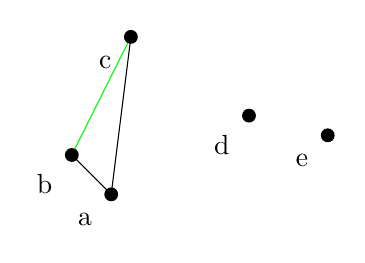
\begin{tikzpicture}[scale=1]
                % Define the coordinates of the points
                \coordinate (a) at (3.25,10.5);
                \coordinate (b) at (2.75,11);
                \coordinate (c) at (3.5,12.5);
                \coordinate (d) at (5,11.5);
                \coordinate (e) at (6,11.25);
                
                % Draw the lines
                \draw (c) -- (a) -- (b);
                \draw[green] (b) -- (c);
    
                \foreach \point/\label in {a/a, b/b, c/c, d/d, e/e}
                    \fill (\point) circle (2.5pt) node[label={below left:\label}] {};
    
            \end{tikzpicture}
        \end{subfigure}
        
        \vspace{30pt}
        
        \begin{subfigure}{0.45\textwidth}
            \centering
            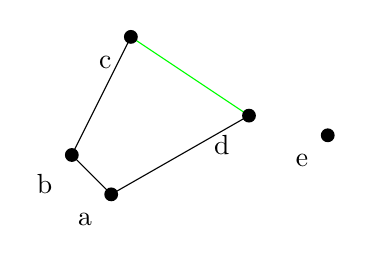
\begin{tikzpicture}[scale=1]
                % Define the coordinates of the points
                \coordinate (a) at (3.25,10.5);
                \coordinate (b) at (2.75,11);
                \coordinate (c) at (3.5,12.5);
                \coordinate (d) at (5,11.5);
                \coordinate (e) at (6,11.25);
                
                \draw (d) -- (a) -- (b) -- (c) ;
                \draw[green] (c) -- (d);
    
                \foreach \point/\label in {a/a, b/b, c/c, d/d, e/e}
                    \fill (\point) circle (2.5pt) node[label={below left:\label}] {};
            \end{tikzpicture}
        \end{subfigure}
        \hfill
        \begin{subfigure}{0.45\textwidth}
            \centering
            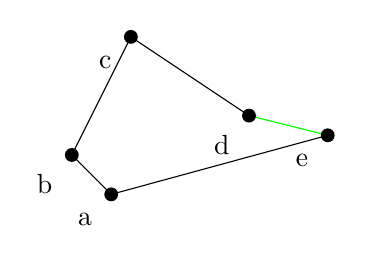
\begin{tikzpicture}[scale=1]
                % Define the coordinates of the points
                \coordinate (a) at (3.25,10.5);
                \coordinate (b) at (2.75,11);
                \coordinate (c) at (3.5,12.5);
                \coordinate (d) at (5,11.5);
                \coordinate (e) at (6,11.25);
                
                \draw (e) -- (a) -- (b) -- (c) -- (d) ;
                \draw[green] (d) -- (e);
    
                \foreach \point/\label in {a/a, b/b, c/c, d/d, e/e}
                    \fill (\point) circle (2.5pt) node[label={below left:\label}] {};
    
            \end{tikzpicture}
        \end{subfigure}
    \end{example}
    \caption{Nearest addition příklad}
\end{figure}

\subsubsection{Aproximační faktor}
\begin{theorem}
Nearest addition  je 2-aproximační algoritmus.
\end{theorem}

Abychom si tvrzení dokázali, musíme si nejdříve ukázat vztah k Primově algoritmu, který hledá minimální kostru grafu.\newline

{\SetAlgoNoLine\
\begin{algorithm}[H]
new list $spanningTree$\;
new list $unvisitedCities$\;
$unvisitedCities \leftarrow nodes$\;
$(i, j) \leftarrow $ shortest edge in graph\;
$spanningTree.Add((i, j))$\;
$unvisitedCities.Remove(i, j)$\;

\While{$unvisitedCities.Count > 0$}{
$(k, l) \leftarrow $ shortest edge in graph, where $k \notin unvisitedCities$ and $l \in unvisitedCities$\;
$spanningTree.Add((k, l))$\;
$unvisitedCities.Remove(l)$\;
}
\Return{$spanningTree$}
\caption{Primův algoritmus}
\end{algorithm}}\leavevmode\newline

Z pseudokódu je jasné, že hrany nalezené Primovým algoritmem i~\mbox{nearest}~\mbox{addition} algoritmem budou totožné.

Zůstaňme ještě chvíli u kostry grafy a jejím vztahu k cestě nalezené TSP~algoritmy.

\begin{lemma}\label{lemma:MSP}
Pro libovolný vstup TSP je cena jeho optimální cesty alespoň tak vysoká, jako je cena minimální kostry pro tentýž vstup.
\end{lemma}

\begin{proof}
Vezměme optimální cestu pro libovolný vstup s více než jedním vrcholem a odstraňme některou z hran. Takto vzniklý graf jistě nebude mít vyšší cenu než optimální cesta. Navíc bude také kostrou původního vstupu. To si můžeme snadno ověřit. Graf stále obsahuje všechny vrcholy, jeho souvislost jsme nijak neporušili a jedinou kružnici kterou obsahoval jsme otevřeli odstraněním jedné z hran.


\begin{center}
	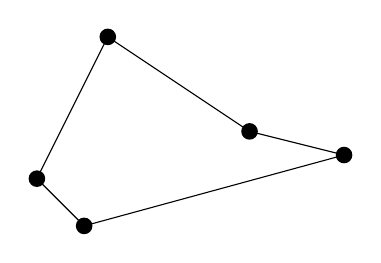
\begin{tikzpicture}[scale=1.2]
		% Define the coordinates of the points
		\coordinate (A) at (3.25,10.5);
		\coordinate (B) at (2.75,11);
		\coordinate (C) at (3.5,12.5);
		\coordinate (D) at (5,11.5);
		\coordinate (E) at (6,11.25);
    
		\foreach \point/\label in {A/A, B/B, C/C, D/D, E/E}
			\fill (\point) circle (2.5pt) node[] {};

		% Draw the lines
		\draw (A) -- (B) -- (C) -- (D) -- (E) -- (A);
	\end{tikzpicture}
  	\hspace{70pt}
	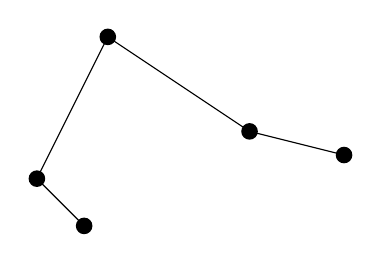
\begin{tikzpicture}[scale=1.2]
		% Define the coordinates of the points
		\coordinate (A) at (3.25,10.5);
		\coordinate (B) at (2.75,11);
		\coordinate (C) at (3.5,12.5);
		\coordinate (D) at (5,11.5);
		\coordinate (E) at (6,11.25);
    
		\foreach \point/\label in {A/A, B/B, C/C, D/D, E/E}
			\fill (\point) circle (2.5pt) node[] {};

		% Draw the lines
		\draw (A) -- (B) -- (C) -- (D) -- (E);
	\end{tikzpicture}
\end{center} 		
\captionof{figure}{Vztah okružní cesty v grafu a jeho kostry}\leavevmode\newline

To, že tato kostra nemůže mít nižší cenu než minimální kostra, je triviální a lemma jsme dokázali.
\end{proof}

\begin{theorem}
Nearest addition algoritmus pro metrický problém obchodního cestujícího je 2-aproximační algoritmus.
\end{theorem}

\begin{proof}
Uvažujme podmnožiny $S_1, S_2,…,S_{n-1}$ hran grafu, kde $S_i$ je množina hran identifikovaných $i$-tou iterací. Vrátíme-li se k příkladu chodu algoritmu, pak ve stavu na obrázku \ref{tikzpicture:naExampleA} bude $S_1 = \{(a, b)\}$, pro stav na \ref{tikzpicture:naExampleB} bude $S_2 = \{(a, b), (b, c)\}$, atd. Dále mějme množinu $F = \{(i_1, j_1), (i_2, j_2), $ $\cdots$ $,(i_{n-1}, j_{n-1})\}$ reprezentující nejkratší hrany určené každým průchodem cyklu (na obrázku zvýrazněné zeleně). Jak bylo zmíněno výše, tato množina bude jistě množinou hran nejkratší kostry vstupního grafu. Tedy z lemma \ref{lemma:MSP} plyne
$$
OPT \ge\sum_{l = 1}^{n-1} c_{i_l j_l}
$$

Po najití první nejkratší hrany máme výslednou délku $c_1 = 2c_{i_1, j_1}$, jelikož ji vkládáme do cesty dvakrát. Dále, když přidáváme nové město $j$ mezi $i$ a $k$, tak rušíme hranu $(i, k)$ a přidáváme hrany $(i, j)$ a $(j, k)$. Cesta se tedy prodlužuje o $c_{ij} + c_{jk} - c_{ik}$. Z trojúhelníkové nerovnosti snadno odvodíme, že $c_{jk} - c_{ik} \le c_{ij}$. Rozdíl cen hran $c_{jk}$ a $c_{ik}$ je tedy shora ohraničený cenou $c_{ij}$.

Dosadíme-li tuto hodnotu do předchozí rovnice, zjistíme, že celková cesta se může v nejhorším případě prodloužit o $2c_{ij}$. Celková cesta nalezená narest addition algoritmem bude tedy maximálně $2\sum_{l=1}^{n-1}c_{i_l j_l}$.

Upravíme li poslední nerovnost, dostaneme $\sum_{l=2}^{n}c_{i_l j_l} \le 2OPT$.

To znamená, že cesta nalezená algoritmem v nejhorším případě stát bude stát nejvýše dvakrát tolik, co optimální cesta pro stejný vstup, což je přesně to, co jsme chtěli dokázat.
\end{proof}

\subsubsection{Tight example} \label{tightExample:NA}

Můžeme si ukázat jeho tzv. \textit{tight example}, což je pro algoritmus s aproximačním faktorem $\alpha$ příklad, u kterého nalezne řešení s cenou $\alpha * OPT$ (můžeme povolit určitou konstantní odchylku). Tedy budeme chtít najít vstup  pro metrický TSP, pro který nám tento algoritmus vrátí cestu s délkou skoro $2 * OPT$.

Vezměme si jako vstup $(n - 1)$-cípou hvězdu s jedním vrcholem ve svém středu. Hrany busou ohodnoceny následovně: hrany vlevo na obrázku budou mít cenu jedna a hrany vpravo dva.


\begin{figure}[H]
    \begin{center}
		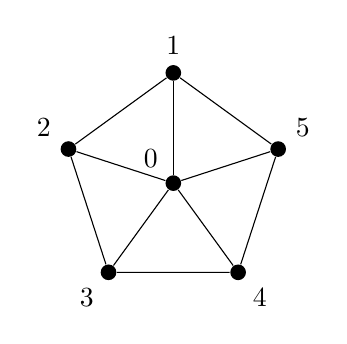
\begin{tikzpicture}[scale=0.7]
 			 % Set the radius of the imaginary circle
 	 		\def\radius{2cm}
  
	  		% Calculate the position of each point on the circle
 	 		\foreach \i in {1,...,5}
 		    	{\draw ({360/5 * (\i - 1) + 90}:\radius) node[circle, fill, inner sep=2pt, label={360/5 * (\i - 1) + 90:${\i}$}] (t\i) {};}
 	 		\draw ({0}:0) node[circle, fill, inner sep=2pt, label={above left:0}] (t0) {};
 	 		
 	 		\draw (t1) -- (t2) -- (t3) -- (t4) -- (t5) -- (t1);
 	 		\draw (t0) -- (t1);
 	 		\draw (t0) -- (t2);
 	 		\draw (t0) -- (t3);
 	 		\draw (t0) -- (t4);
 	 		\draw (t0) -- (t5);
		\end{tikzpicture}
		\hspace{75pt}
		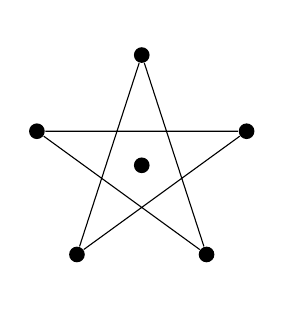
\begin{tikzpicture}[scale=0.7]
 			 % Set the radius of the imaginary circle
 	 		\def\radius{2cm}
  
	  		% Calculate the position of each point on the circle
 	 		\foreach \i in {1,...,5}
 		    	{\draw ({360/5 * (\i - 1) + 90}:\radius) node[circle, fill, inner sep=2pt, label={}] (t\i) {};} 	 	
 	 		\draw ({0}:0) node[circle, fill, inner sep=2pt, label={}] (t0) {};
 	 		
 	 		\draw (t1) -- (t3) -- (t5) -- (t2) -- (t4) -- (t1);
 	 		
 	 		\node[below, white] at (current bounding box.south) {0};
		\end{tikzpicture}
    \end{center}
    \caption{Nearest addition tight example}
\end{figure}

Cena hran napravo je shora omezená právě dva, protože musí platit trojúhelníková nerovnost.

\begin{figure}[H]
    \begin{center}
		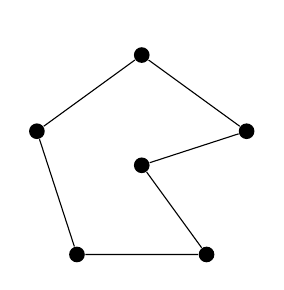
\begin{tikzpicture}[scale=0.7]
 			 % Set the radius of the imaginary circle
 	 		\def\radius{2cm}
  
	  		% Calculate the position of each point on the circle
 	 		\foreach \i in {1,...,5}
 		    	{\draw ({360/5 * (\i - 1) + 90}:\radius) node[circle, fill, inner sep=2pt, label={}] (t\i) {};} 	 	
 	 		\draw ({0}:0) node[circle, fill, inner sep=2pt, label={}] (t0) {};
 	 		
 	 		\draw (t5) -- (t1) -- (t2) -- (t3) -- (t4) -- (t0) -- (t5);
		\end{tikzpicture}
		\hspace{75pt}
		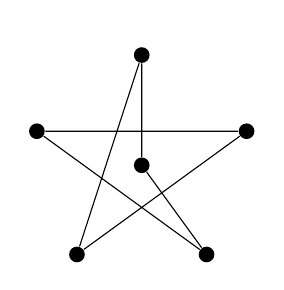
\begin{tikzpicture}[scale=0.7]
 			 % Set the radius of the imaginary circle
 	 		\def\radius{2cm}
  
	  		% Calculate the position of each point on the circle
 	 		\foreach \i in {1,...,5}
 		    	{\draw ({360/5 * (\i - 1) + 90}:\radius) node[circle, fill, inner sep=2pt, label={}] (t\i) {};} 	 	
 	 		\draw ({0}:0) node[circle, fill, inner sep=2pt, label={}] (t0) {};
 	 		
 	 		\draw (t1) -- (t3) -- (t5) -- (t2) -- (t4)-- (t0) -- (t1);
		\end{tikzpicture}
    \end{center}
    \caption{Nearest addition tight example - cesty}
\end{figure}

Je snadno vidět, že optimální cesta (na obrázku výše vlevo) bude mít celkovou cenu $n$.  Algoritmem ale může být nalezena i cesta jako na obrázku nahoře vpravo (příklad chodu algoritmu je zobrazen níže). Taková cesta obsahuje $n-2$  hran s~vahou dva a dvě hrany s vahou jedna, tedy $2(n - 2) + 2 = 2n - 2 = 2*OPT - O(1)$.

\begin{figure}[H]
    \begin{center}
		\begin{tikzpicture}[scale=0.57]
 			 % Set the radius of the imaginary circle
 	 		\def\radius{2cm}
  
	  		% Calculate the position of each point on the circle
 	 		\foreach \i in {1,...,5}
 		    	{\draw ({360/5 * (\i - 1) + 90}:\radius) node[circle, fill, inner sep=1.5pt, label={}] (t\i) {};} 	 	
 	 		\draw ({0}:0) node[circle, fill, inner sep=1.5pt, label={}] (t0) {};
 	 		
 	 		\draw (t0) to[out=75, in=-75] (t1);
 	 		\draw (t0) to[out=105, in=-105] (t1);
 	 		
        	\node[below=7mm] at (current bounding box.south) {\footnotesize 0, \textbf{1}, 0};
		\end{tikzpicture}
		\hspace{4pt}
		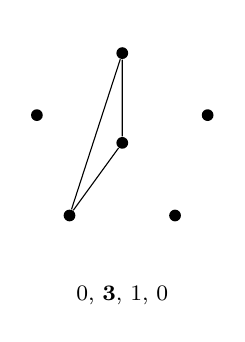
\begin{tikzpicture}[scale=0.57]
 			 % Set the radius of the imaginary circle
 	 		\def\radius{2cm}
  
	  		% Calculate the position of each point on the circle
 	 		\foreach \i in {1,...,5}
 		    	{\draw ({360/5 * (\i - 1) + 90}:\radius) node[circle, fill, inner sep=1.5pt, label={}] (t\i) {};} 	 	
 	 		\draw ({0}:0) node[circle, fill, inner sep=1.5pt, label={}] (t0) {};
 	 		
 	 		\draw (t0) -- (t3) -- (t1) -- (t0);
 	 		
        	\node[below=7mm] at (current bounding box.south) {\footnotesize 0, \textbf{3}, 1, 0};
		\end{tikzpicture}
		\hspace{4pt}
		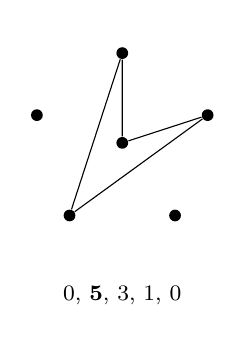
\begin{tikzpicture}[scale=0.57]
 			 % Set the radius of the imaginary circle
 	 		\def\radius{2cm}
  
	  		% Calculate the position of each point on the circle
 	 		\foreach \i in {1,...,5}
 		    	{\draw ({360/5 * (\i - 1) + 90}:\radius) node[circle, fill, inner sep=1.5pt, label={}] (t\i) {};} 	 	
 	 		\draw ({0}:0) node[circle, fill, inner sep=1.5pt, label={}] (t0) {};
 	 		
 	 		\draw (t0) -- (t5) -- (t3) -- (t1) -- (t0);
 	 		
        	\node[below=7mm] at (current bounding box.south) {\footnotesize 0, \textbf{5}, 3, 1, 0};
		\end{tikzpicture}
		\hspace{4pt}
		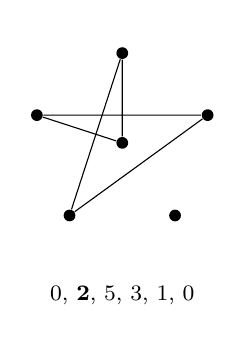
\begin{tikzpicture}[scale=0.57]
 			 % Set the radius of the imaginary circle
 	 		\def\radius{2cm}
  
	  		% Calculate the position of each point on the circle
 	 		\foreach \i in {1,...,5}
 		    	{\draw ({360/5 * (\i - 1) + 90}:\radius) node[circle, fill, inner sep=1.5pt, label={}] (t\i) {};} 	 	
 	 		\draw ({0}:0) node[circle, fill, inner sep=1.5pt, label={}] (t0) {};
 	 		
 	 		\draw (t0) -- (t2) -- (t5) -- (t3) -- (t1) -- (t0);
 	 		
        	\node[below=7mm] at (current bounding box.south) {\footnotesize 0, \textbf{2}, 5, 3, 1, 0};
		\end{tikzpicture}
		\hspace{4pt}
		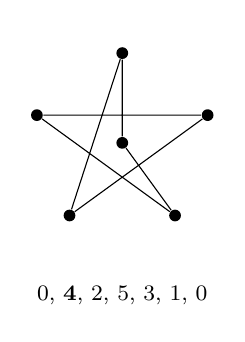
\begin{tikzpicture}[scale=0.57]
 			 % Set the radius of the imaginary circle
 	 		\def\radius{2cm}
  
	  		% Calculate the position of each point on the circle
 	 		\foreach \i in {1,...,5}
 		    	{\draw ({360/5 * (\i - 1) + 90}:\radius) node[circle, fill, inner sep=1.5pt, label={}] (t\i) {};} 	 	
 	 		\draw ({0}:0) node[circle, fill, inner sep=1.5pt, label={}] (t0) {};
 	 		
 	 		\draw (t0) -- (t4) -- (t2) -- (t5) -- (t3) -- (t1) -- (t0);
 	 		
        	\node[below=7mm] at (current bounding box.south) {\footnotesize 0, \textbf{4}, 2, 5, 3, 1, 0};
		\end{tikzpicture}
    \end{center}
    \caption{Nearest addition tight example - chod algoritmu}
\end{figure}

\subsection{Double-tree}
Jádrem algoritmu je zdvojení hran minimální kostry vstupního grafu a následné nalezení uzavřeného eulerovského tahu. To, že se v takovémto grafu takový tah nachází je snadné dokázat. Z Věty \ref{theorem:eulerianCircout} víme, že stačí, aby byl graf spojitý a všechny jeho uzly měly sudý stupeň. Zdvojíme-li každou hranu, vycházející z libovolného uzlu, pak bude mít jistě uzel sudý stupeň. Jelikož vycházíme z kostry grafu, spojitost je zřejmá.

K vytvoření cesty už potřebujeme pouze zaručit, že nenavštívíme žádný uzel vícekrát. Toho dosáhneme pomocí zkracování. Máme-li eulerovský průchod $(i_0, i_1)$, $(i_1, i_2)$, $\cdots$ $(i_{k-1}, i_k)$, $(i_k, i_0)$, pak vezměme posloupnost $i_0, i_1,... i_k$ a ponechejme pro každý uzel pouze jeho první výskyt. Nakonec ještě vraťme $i_0$ na konec cesty. \newline

{\SetAlgoNoLine\
\begin{algorithm}[H]
\KwIn{G}
$doubleTree \leftarrow FindMinimalSpanningTree(G)$\;
\ForEach{$edge \in doubleTree$}
{
	$doubleTree.Add(edge)$\;
}
$eulerCircuit \leftarrow FindEulerCircuit(doubleTree)$\;
vytvoř seznam $path$\;
\ForEach{$node \in eulerCircuit$}
{
	\If{$node \not \in path$}
	{
		$path.Add(node)$\;
	}
}
\Return{$path$}
\caption{Double-tree algoritmus}
\end{algorithm}}\leavevmode\newline

\begin{figure}[H]
    \begin{example}
    \leavevmode\newline
    \begin{tikzpicture}[scale=1]
		% Define the coordinates of the points
		\coordinate (a) at (0,1);
		\coordinate (b) at (1,0.75);
		\coordinate (c) at (1.5,0);
  		\coordinate (d) at (2,2.5);
        \coordinate (e) at (2.75,2.4);
                
        % Draw the lines
        \draw (a) -- (b) -- (c);
        \draw (b) -- (d) -- (e);
    
        \foreach \point/\label in {a/a, b/b, c/c}
        \fill (\point) circle (2.5pt) node[label={below left:\label}] {};
    
        \foreach \point/\label in  {d/d, e/e}
        \fill (\point) circle (2.5pt) node[label={above:\label}] { };
        
        \node[below, white] at (current bounding box.south) {a, b, c, d, e};
     \end{tikzpicture}
     \hfill
     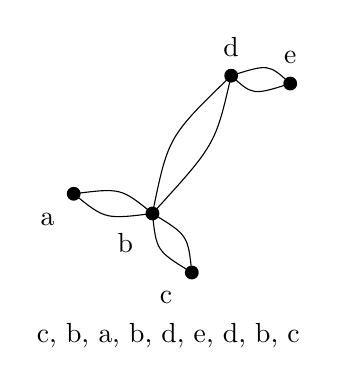
\begin{tikzpicture}[scale=1]
		 % Define the coordinates of the points
		\coordinate (a) at (0,1);
		\coordinate (b) at (1,0.75);
		\coordinate (c) at (1.5,0);
  		\coordinate (d) at (2,2.5);
        \coordinate (e) at (2.75,2.4);
                
         % Draw the lines
        % Draw the lines
        \draw (a) .. controls ($(a)!0.5!(b) + (0.1, 0.2)$) and ($(a)!0.5!(b) + (0.1, 0.2)$) .. (b);
        \draw (a) .. controls ($(a)!0.5!(b) - (0.1, 0.2)$) and ($(a)!0.5!(b) - (0.1, 0.2)$) .. (b);
        \draw (b) .. controls ($(b)!0.5!(c) + (0.2, 0.1)$) and ($(b)!0.5!(c) + (0.2, 0.1)$) .. (c);
        \draw (b) .. controls ($(b)!0.5!(c) - (0.2, 0.1)$) and ($(b)!0.5!(c) - (0.2, 0.1)$) .. (c);
        \draw (b) .. controls ($(b)!0.5!(d) + (0.3, 0)$) and ($(b)!0.5!(d) + (0.3, 0)$) .. (d);
        \draw (b) .. controls ($(b)!0.5!(d) - (0.3, -0.1)$) and ($(b)!0.5!(d) - (0.3, -0.1)$) .. (d);
        \draw (d) .. controls ($(d)!0.5!(e) + (0.1, 0.2)$) and ($(d)!0.5!(e) + (0.1, 0.2)$) .. (e);
        \draw (d) .. controls ($(d)!0.5!(e) - (0.1, 0.2)$) and ($(d)!0.5!(e) - (0.1, 0.2)$) .. (e);
    
        \foreach \point/\label in {a/a, b/b, c/c}
        \fill (\point) circle (2.5pt) node[label={below left:\label}] {};
    
        \foreach \point/\label in  {d/d, e/e}
        \fill (\point) circle (2.5pt) node[label={above:\label}] {};
        
        \node[below] at (current bounding box.south) {c, b, a, b, d, e, d, b, c};
      \end{tikzpicture}
      \hfill
      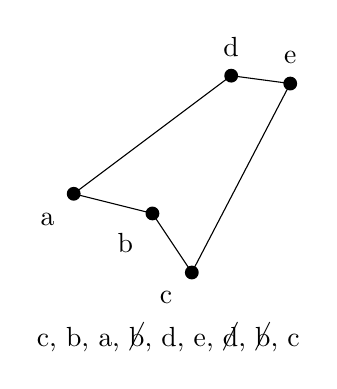
\begin{tikzpicture}[scale=1]
		 % Define the coordinates of the points
		\coordinate (a) at (0,1);
		\coordinate (b) at (1,0.75);
		\coordinate (c) at (1.5,0);
  		\coordinate (d) at (2,2.5);
        \coordinate (e) at (2.75,2.4);
                
         % Draw the lines
         \draw (a) -- (b) -- (c) -- (e) -- (d) -- cycle;
    
        \foreach \point/\label in {a/a, b/b, c/c}
        \fill (\point) circle (2.5pt) node[label={below left:\label}] {};
    
        \foreach \point/\label in  {d/d, e/e}
        \fill (\point) circle (2.5pt) node[label={above:\label}] {};
        \node[below] at (current bounding box.south) {c, b, a, \cancel{b}, d, e, \cancel{d}, \cancel{b}, c};
      \end{tikzpicture}
    \end{example}
    \caption{Double-tree příklad}
\end{figure}


\subsubsection{Aproximační faktor}
\begin{theorem}
Double-tree je 2-aproximační algoritmus.
\end{theorem}
	Z Lemma \ref{lemma:MSP} víme, že optimální cesta stojí alespoň tolik, co minimální kostra. Jelikož každou její hranu zdvojujeme, získáme dvakrát tak delší cestu.
	
	Při hledání eulerovského průchodu pouze hrany seřazujeme.
	
	Zbývá pouze zkracování. Zde opět vycházíme z trojúhelníkové nerovnosti. Uvažujme, že $i$, $j$, $k$ jsou po sobě jdoucí města a $j$ jsme již navštívili, tedy bychom je měli přeskočit. Je zřejmé, že $c_{ij} + c_{jk} \ge c_{ik}$ , což dokazuje, cena tohoto úseku zůstane při nejhorším stejná a horní ohraničení se tedy nemění.
	
\subsubsection{Tight example}
Jako příklad vstupu, pro který double-tree algortimus najde cestu délky $2OPT$ můžeme vzít vstup z kapitoly \ref{tightExample:NA} o nearest addition algoritmu. Jelikož mají oba algoritmy stejný aproximační faktor, pak stačí ukázat, že se můžeme double-tree algoritmem dostat ke stejné cestě jako v již zmíněné předchozí kapitole.

U takového vstupu může být nalezena následná minimální kostra.

\begin{figure}[H]
    \begin{center}
		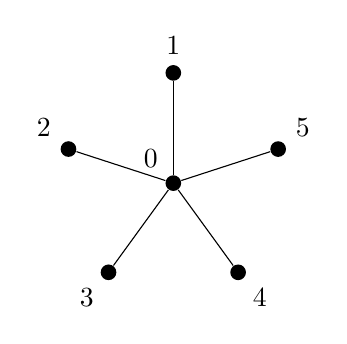
\begin{tikzpicture}[scale=0.7]
 			 % Set the radius of the imaginary circle
 	 		\def\radius{2cm}
  
	  		% Calculate the position of each point on the circle
 	 		\foreach \i in {1,...,5}
 		    	{\draw ({360/5 * (\i - 1) + 90}:\radius) node[circle, fill, inner sep=2pt, label={360/5 * (\i - 1) + 90:${\i}$}] (t\i) {};}
 	 		\draw ({0}:0) node[circle, fill, inner sep=2pt, label={above left:0}] (t0) {};
 	 		
 	 		\draw (t0) -- (t1);
 	 		\draw (t0) -- (t2);
 	 		\draw (t0) -- (t3);
 	 		\draw (t0) -- (t4);
 	 		\draw (t0) -- (t5);
		\end{tikzpicture}
    \caption{Double tree tight example - minimální kostra}
    \end{center}
\end{figure}

V grafu se zdvojenými hranami, pak můžeme uvažovat eulerovský průchod 0,~4, 0, 2, 0, 5, 0, 3, 0, 1, 0, ze kterého zkrácením dostaneme cestu 0, 4, 2, 5, 3, 1, 0, což je stejná cesta jakou jsme nalezli algoritmem nearest addition.

\subsection{Christofides'}
Christofidesův algoritmus je velice podobný double-tree algoritmu. Opět \mbox{začneme} s minimální kostrou vstupního grafu. Existenci eulerovského průchodu ale~\mbox{zajistíme} o něco chytřeji. Připomeňme si, že eulerovský průchod se v grafu nachází právě tehdy, když mají všechny jeho uzly sudý stupeň. V double-tree algoritmu jsme tuto podmínku splnili tak, že jsme zdvojili každou hranu kostry. To je ovšem redundantní. Postačí, když spárujeme takové její uzly, které mají lichý stupeň.

Mějme úplný graf, jehož množinou vrcholů budou právě ty vrcholy jeho minimální kostry s lichým stupněm, označme ji $O$. Z množiny jeho hran se budeme snažit vybrat takovou podmnožinu, ve které bude $\forall v \in O$ právě jedna hrana, pro kterou je $v$ koncový uzel. Taková množina se nazývá \textit{perfektní párování}. Na~\mbox{množině} jich samozřejmě může být více. Pro naše účely bude jistě nejlepší hledat takovou z nich, která budeme mít minimální součet délek všech svých hran, tedy \textit{minimální perfektní párování}. K jeho nalezení se v programu používá C++ knihovna Vladimira Kolmogorova, která implementuje $Blossom~V$ algoritmus.

Uvědomme si ale, že aby takové párování pro $O$ existovalo, tak musí být $|O|$ sudé. Víme, že součet stupňů všech uzlů v neorientovaném grafu je sudé číslo (viz Věta \ref{theorem:degree}). Označme si množinu všech vrcholů grafu $V$ a množinu vrcholů se~sudým stupněm $E$. Jistě platí
$$
\sum_{v \in V} deg(v) = \sum_{v \in E} deg(v) + \sum_{v \in O} deg(v)
$$

$\sum_{v \in V} deg(v)$ je ale určitě sudé a to samé platí pro $\sum?_{v \in E}$, tedy $\sum_{v \in O} deg(v)$ musí být také sudý. Vzhledem k tomu, že každý vrchol přispívá do součtu lichým číslem, pak musí být sudý jejich počet.

Přidáním minimálního perfektního párování k minimální kostře zvýšíme stupeň každého vrcholu s lichým stupněm právě o jedna, tudíž zajistíme, že~všechny uzly budou mít sudý stupeň. V takovém grafu pak existuje uzavřený eulerovský tah. Po jeho nalezení už jen zkracujeme cestu stejným způsobem jako u double-tree algoritmu.\leavevmode\newline

{\SetAlgoNoLine\
\begin{algorithm}[H]
\KwIn{G}
$spanningTree \leftarrow FindMinimalSpanningTree(G)$\;
$oddDegreeNodes \leftarrow FindNodesWithOddDegrees(spanningTree)$;
$perfectMathing \leftarrow FindPerfectMatching(oddDegreeNodes)$;
$eulerCircuit \leftarrow FindEulerCircuit(doubleTree + perfectMathing)$\;
vytvoř seznam $path$\;
\ForEach{$node \in eulerCircuit$}
{
	\If{$node \not \in path$}
	{
		$path.Add(node)$\;
	}
}
\Return{$path$}
\caption{Christofidesův algoritmus}
\end{algorithm}}\leavevmode\newline

\begin{figure}[H]
    \begin{example}
    \leavevmode\newline
    \begin{tikzpicture}[scale=1]
		% Define the coordinates of the points
		\coordinate (a) at (0,1);
		\coordinate (b) at (1,0.75);
		\coordinate (c) at (1.5,0);
  		\coordinate (d) at (2,2.5);
        \coordinate (e) at (2.75,2.4);
                
        % Draw the lines
        \draw (a) -- (b) -- (c);
        \draw (b) -- (d) -- (e);
    
        \foreach \point/\label in {a/a, c/c}
        \fill[blue] (\point) circle (2.5pt) node[label={below left:\label}] {};
        
        \fill[blue] (b) circle (2.5pt) node[label={above left:b}] {};
        \fill (d) circle (2.5pt) node[label={above:d}] {};
        \fill[blue] (e) circle (2.5pt) node[label={above:e}] {};
        
        \node[below, white] at (current bounding box.south) {a, b, c, d, e};
     \end{tikzpicture}
     \hfill
     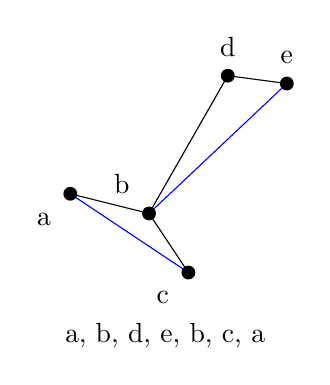
\begin{tikzpicture}[scale=1]
		 % Define the coordinates of the points
		\coordinate (a) at (0,1);
		\coordinate (b) at (1,0.75);
		\coordinate (c) at (1.5,0);
  		\coordinate (d) at (2,2.5);
        \coordinate (e) at (2.75,2.4);
                
        % Draw the lines
        \draw (a) -- (b) -- (c) -- (b) -- (d) -- (e);
        \draw[blue] (a) -- (c);
        \draw[blue] (b) -- (e);
    
        \foreach \point/\label in {a/a, c/c}
        \fill (\point) circle (2.5pt) node[label={below left:\label}] {};
    
        \fill (b) circle (2.5pt) node[label={above left:b}] {};
        
        \foreach \point/\label in  {d/d, e/e}
        \fill (\point) circle (2.5pt) node[label={above:\label}] {};
        
        \node[below] at (current bounding box.south) {a, b, d, e, b, c, a};
      \end{tikzpicture}
      \hfill
      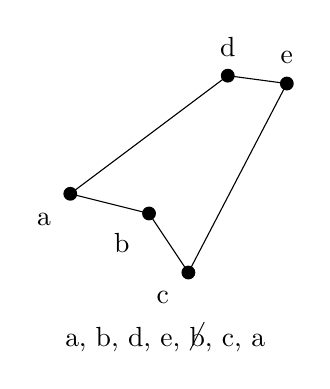
\begin{tikzpicture}[scale=1]
		 % Define the coordinates of the points
		\coordinate (a) at (0,1);
		\coordinate (b) at (1,0.75);
		\coordinate (c) at (1.5,0);
  		\coordinate (d) at (2,2.5);
        \coordinate (e) at (2.75,2.4);
                
         % Draw the lines
         \draw (a) -- (b) -- (c) -- (e) -- (d) -- cycle;
    
        \foreach \point/\label in {a/a, b/b, c/c}
        \fill (\point) circle (2.5pt) node[label={below left:\label}] {};
    
        \foreach \point/\label in  {d/d, e/e}
        \fill (\point) circle (2.5pt) node[label={above:\label}] {};
        \node[below] at (current bounding box.south) {a, b, d, e, \cancel{b}, c, a};
      \end{tikzpicture}
    \end{example}
    \caption{Christofides' příklad}
\end{figure}

\subsubsection{Aproximační faktor}
\begin{theorem}
	Christofidesův algoritmus  je 3/2-aproximační algoritmus.
\end{theorem}

	Nejdřív si musíme rozmyslet, co vlastně potřebujeme dokázat. Potřebujeme, aby eulerovský průchod měl při nejhorším délku $\frac{3}{2}OPT$. Z lemmatu \ref{lemma:MSP} víme, že minimální kostra, která je v něm obsažená, má v nejhorším případě cenu OPT. Stačí tedy dokázat, že perfektní párování má maximálně cenu $\frac{1}{2} OPT$.
	
	Pracujeme s množinou lichých uzlů v MST $O$. Budeme v ní teď hledat cestu. Vyjdeme-li z nejkratší cesty nad všemi vrcholy vstupu, pak je zřejmé, že její délka bude nejvýše $OPT$. Tuto cestu teď budeme pouze zkracovat. Uvažujeme-li dvě města $i$ a $j$, pro která platí, že na cestě mezi nimi jsou pouze města nenáležící do $O$, pak je jistě můžeme vynechat a z trojúhelníkové nerovnosti víme, že v nejhorším případě bude hrana $(i,j)$ stejně dlouhá jako původní cesta. V nejhorším případě tedy po tomto zkracování zůstane délka cesty rovna $OPT$.
	
	Nyní začněme střídavě obarvovat hrany nalezené cesty, řekněme modrou a červenou. Množina červených i množina modrých hran je perfektním párováním na $O$, platí totiž, že pokrývají všechny vrcholy a žádné dvě hrany nesdílí vrchol. Víme, že dohromady množiny dávají $OPT$, pak jistě jedna z množin bude mít délka menší nebo rovnu $\frac{1}{2}OPT$, což jsme chtěli dokázat.

\begin{figure}[H]
    \leavevmode\newline
    \begin{tikzpicture}[scale=1]
		% Define the coordinates of the points
		\coordinate (a) at (0,1);
		\coordinate (b) at (1,0.75);
		\coordinate (c) at (1.5,0);
  		\coordinate (d) at (2,2.5);
        \coordinate (e) at (2.75,2.4);
                
        % Draw the lines
        \draw (a) -- (b) -- (c);
        \draw (b) -- (d) -- (e);
    
        \foreach \point/\label in {a/a, c/c}
        \fill[blue] (\point) circle (2.5pt) node[label={below left:\label}] {};
        
        \fill[blue] (b) circle (2.5pt) node[label={above left:b}] {};
        \fill (d) circle (2.5pt) node[label={above:d}] {};
        \fill[blue] (e) circle (2.5pt) node[label={above:e}] {};
     \end{tikzpicture}
     \hfill
     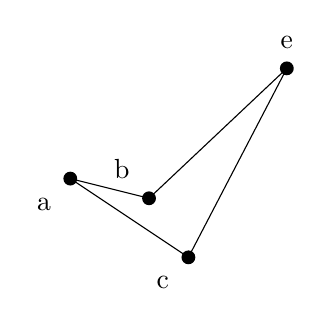
\begin{tikzpicture}[scale=1]
		 % Define the coordinates of the points
		\coordinate (a) at (0,1);
		\coordinate (b) at (1,0.75);
		\coordinate (c) at (1.5,0);
  		\coordinate (d) at (2,2.5);
        \coordinate (e) at (2.75,2.4);
                
        % Draw the lines
        \draw (a) -- (b);
        \draw (c) -- (a);
        \draw (e) -- (c);
        \draw (e) -- (b);
    
        \foreach \point/\label in {a/a, c/c}
        \fill (\point) circle (2.5pt) node[label={below left:\label}] {};
        
        \fill (b) circle (2.5pt) node[label={above left:b}] {};
        \fill (e) circle (2.5pt) node[label={above:e}] {};
      \end{tikzpicture}
      \hfill
      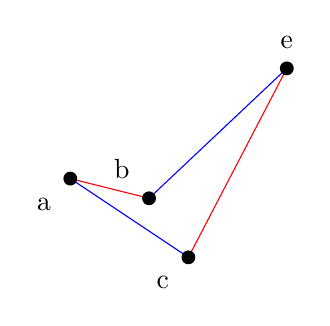
\begin{tikzpicture}[scale=1]
		 % Define the coordinates of the points
		\coordinate (a) at (0,1);
		\coordinate (b) at (1,0.75);
		\coordinate (c) at (1.5,0);
  		\coordinate (d) at (2,2.5);
        \coordinate (e) at (2.75,2.4);
                
        % Draw the lines
        \draw[red] (a) -- (b);
        \draw[blue] (c) -- (a);
        \draw[red] (e) -- (c);
        \draw[blue](e) -- (b);
    
        \foreach \point/\label in {a/a, c/c}
        \fill (\point) circle (2.5pt) node[label={below left:\label}] {};
        
        \fill (b) circle (2.5pt) node[label={above left:b}] {};
        \fill (e) circle (2.5pt) node[label={above:e}] {};
      \end{tikzpicture}
    \caption{Perfektní párování}
\end{figure}

	
	Z analýz aproximačních faktorů Christofidesova a double-tree algoritmů ještě vyplývá následující tvrzení.
\begin{lemma}
Sestrojíme-li pro vstup eulerovský podgraf délky $\alpha*OPT$, pak můžeme odvodit $\alpha$-aproximační algoritmus.
\end{lemma}

\subsubsection{Tight example}
Vezměme si následující vstup, kde mají vyznačené hrany délku 1.

\begin{figure}[H]
    \begin{center}
            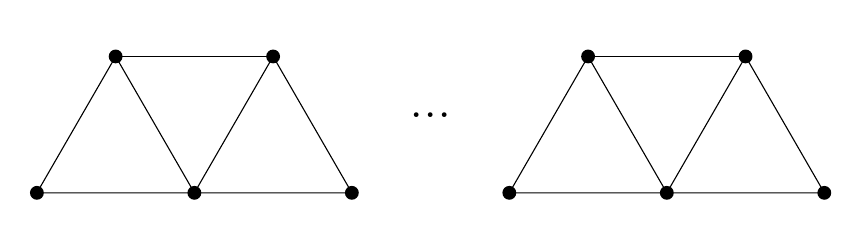
\begin{tikzpicture}[scale=1]
			% Define the coordinates of the points
			\coordinate (a) at (0,0);
			\coordinate (b) at (2,0);
			\coordinate (c) at (1,1.73206);
			\coordinate (d) at (4,0);
			\coordinate (e) at (3,1.73206);
			
			\coordinate (f) at (0+6,0);
			\coordinate (g) at (2+6,0);
			\coordinate (h) at (1+6,1.73206);
			\coordinate (i) at (4+6,0);
			\coordinate (j) at (3+6,1.73206);
                
        	% Draw the lines
        	\draw (a) -- (c) -- (b) -- (e) -- (d) -- (a);
        	\draw (c) -- (e);
        	\draw (f) -- (h) -- (g) -- (j) -- (i) -- (f);
        	\draw (h) -- (j);
    
        	\foreach \point/\label in {a/a, b/b, c/c, d/d, e/e, f/f, g/g, h/h, i/i, j/j}
        	\fill (\point) circle (2.5pt) node[label={}] {};
        	\node[font=\huge] at (current bounding box.center) {...};
            \end{tikzpicture}
    \end{center}
    \caption{Christofides' tight example}
\end{figure}

Bude-li nalezena minimální kostra grafu zobrazená černými hranami na obrázku níže, pak jediné uzly s lichým stupněm budou krajní zobrazené modře. Jejich spojením pak dostanem cestu (zkracování zde jistě nepovede k žádnému zlepšení).

\begin{figure}[H]
        \begin{center}
            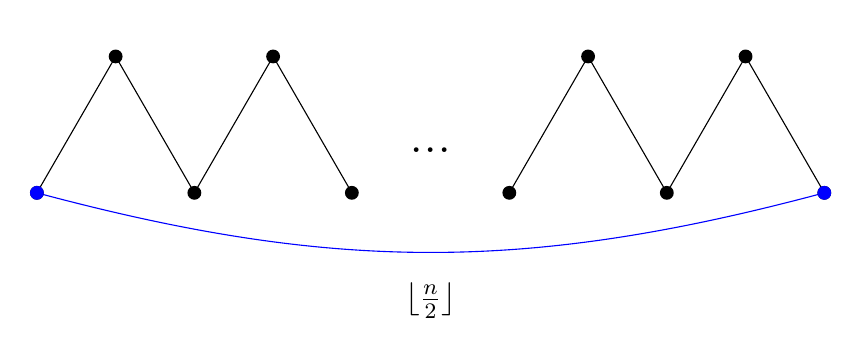
\begin{tikzpicture}[scale=1]
			% Define the coordinates of the points
			\coordinate (a) at (0,0);
			\coordinate (b) at (2,0);
			\coordinate (c) at (1,1.73206);
			\coordinate (d) at (4,0);
			\coordinate (e) at (3,1.73206);
			
			\coordinate (f) at (0+6,0);
			\coordinate (g) at (2+6,0);
			\coordinate (h) at (1+6,1.73206);
			\coordinate (i) at (4+6,0);
			\coordinate (j) at (3+6,1.73206);
                
        	% Draw the lines
        	\draw (a) -- (c) -- (b) -- (e) -- (d);
        	\draw (f) -- (h) -- (g) -- (j) -- (i);
        	\draw (a)[blue] to[out=-15, in=195] (i);
    
        	\foreach \point/\label in {a/a, b/b, c/c, d/d, e/e, f/f, g/g, h/h, i/i, j/j}
        	\fill (\point) circle (2.5pt) node[label={}] {};
        	
        	\fill[blue] (a) circle (2.5pt) node[label={}] {};
        	\fill[blue] (i) circle (2.5pt) node[label={}] {};
        	
        	\node[font=\huge] at (current bounding box.center) {...};
        	\node[below, font=\large] at (current bounding box.south) {$\lfloor \frac{n}{2} \rfloor$};
            \end{tikzpicture}
        \end{center}
    \caption{Christofides' tight example - cesta}
\end{figure}

Podívejme se na délku takto nalezené cesty. Kostra bude mít jistě délku $n - 1$ a poslední přidaná hrana $\lfloor \frac{n}{2} \rfloor$. Je také snadno vidět, že optimální cesta bude délky $n$. Pak už snadno $$(n - 1) + \lfloor \frac{n}{2} \rfloor = n - O(1) = OPT - O(1)$$

\subsection{Keringhan - Lin}

Tento heuristický algoritmus není specifický pro TSP, ale je možné jím řešit obecně problémy, kde máme nějakou podmínku $C$, kterou musejí splňovat jejich řešení, a funkci $f$, která takovým řešením přiřazuje určitou hodnotu. Zadanou pak máme množinu $S$, ve které hledáme podmnožinu $T$, která bude nejen splňovat podmínku $C$, ale její hodnota $f$ bude mezi všemi vyhovujícími podmnožinami minimální. Takové problémy mívají často exponenciální složitost, proto se zpravidla spokojíme s hledáním takových podmnožin, které splňují $C$ a jejich hodnota $f$ je dostatečně malá. Jedním z takových problémů, kde se Kernighan - Lin využívá je například \textit{dělení grafů}. 

Základní myšlenkou je postupné zlepšování úvodního řešení. Hledá se vždy lokální optimum, které se, pokud přinese nějaký zisk (zmenšení hodnoty $f$), použije pro další iteraci.

Na začátku se zvolí pseudonáhodné přípustné řešení $T \subseteq S$ a následně začne cyklus, kde se snažíme $T$ transformovat na jiné platné řešení $T'$. Pokud by platilo $f(T') < f(T)$, pak se $T'$ použije pro další iteraci. V momentě, kdy už nenacházíme řešení, které by přinášely nějaký zisk, tak bylo nalezeno lokálně optimální řešení. V tuto chvíli se buď může skončit nebo se vygeneruje nové počáteční řešení a~proces provést znovu.

\sloppy Samotná transformace probíhá tak, že se hledají takové dvě množiny $\{{x_1, x_2, ..., x_k\} \in T}$ a $\{y_1, y_2, ..., y_k\} \in S - T$, pro které platí, že když nahradíme prvky první množiny v $T$ prvky druhé množiny, pak dostaneme platné řešení $T'$. O tom, jak přijdeme k číslu $k$ bude ještě řeč později.

Idea algoritmu tedy spočívá v tom, že pro pseudonáhodné počáteční řešení najdeme budeme nacházet lokální optima a mezi nimi by se snad mělo objevit i~optimum globální (nebo alespoň řešení se schůdnou hodnotou pro $f$). Přirozeně budeme považovat algoritmus za tím kvalitnější, čím menší počet různých lokálních optim dostaneme a čím větší počet náhodných počátečních řešení nás dovede k dostatečně dobrému výsledku.

Obecná podoba heuristiky by se dala zapsat následovně:\newline


{\LinesNumbered\SetAlgoNoLine\
\begin{algorithm}[H]
$T \leftarrow$ pseudonáhodné řešení\;
$T' \leftarrow$ $T$\;
\While{$T'$}
{
	$T' \leftarrow$ tranformace $T$ taková, že $f(T') < f(T)$\;
}
\Return $T'$ or start over if desired\;
\caption{Keringhan - Lin algoritmus - obecně}
\end{algorithm}
}\leavevmode\newline

Vraťme se ještě ke zmíněnému koeficientu $k$. Jednou z možností, jak nad $k$ uvažovat je jako na předem zvolené číslo. Toho pro řešení TSP využil A. Croes s~$k = 2$ a později S. Lin s $k = 3$. Tento přístup s sebou nese jistá úskalí a to hlavně správnou volbu $k$. S narůstající hodnotou se výrazně zvyšuje i výpočetní čas, ale~přirozeně dostáváme lepší řešení. Zjistit pak, jaké číslo nám zajistí dostatečně dobré výsledky ve schůdném čase, je náročné.

Tomuto problému se můžeme vyhnout tím, že $k$ nebude mít žádnou pevně danou hodnotu. Takového způsobu se bude využívat v naší podobě algoritmu. Jelikož $k$ nebude známé, nemůžeme již jednoduše uvažovat všechny podmnožiny $T$ o velikosti $k$, jako u předchozí varianty. Na místo toho budeme iterativně hledat vždy nejvýhodnější $x_i$ a $y_i$ pro výměnu, budeme si zaznamenávat, pro jaké $i$ byl zisk nejvyšší a až když žádné zlepšení nebude moct být nalezeno, vyměníme příslušné množiny.
\newline

{\LinesNumbered\SetAlgoNoLine\
\begin{algorithm}[H]
\SetKwRepeat{Do}{do}{while}%
$T \leftarrow$ pseudorandom solution\;
\Do {$f(T') > f(T)$}
{
$i \leftarrow 0$\;
$T \leftarrow T'$\;
\While {improvement can be found}
{
$i \leftarrow i + 1$\;
$(x_i, y_i) \leftarrow$ best pair for exchange\;
$G_i \leftarrow$ total gain for $\{x_1, x_2, ..., x_k\}$ and $\{y_1, y_2, ..., y_k\}$\;
}
$k \leftarrow i$, where $G_i$ is max \tcp*[h]{(definition of $G_i$ is below)}\;
$T' \leftarrow (T - \{x_1, x_2, ..., x_k\}) \cup \{y_1, y_2, ..., y_k\}$\;
}
\Return $T'$\;
\caption{Keringhan - Lin algoritmus - variabilní $k$}
\end{algorithm}
}\leavevmode\newline

\leavevmode\newline\leavevmode\newline
Pro takový přístup vyvstává pár pravidel a otázek, které si budeme muset zodpovědět.

Prvním pravidlem je \textit{pravidlo disjunkce}. Budeme požadovat, aby množiny $\{x_1, x_2, ..., x_k\}$ a $\{y_1, y_2, ..., y_k\}$ nesdílely žádné prvky a zbytečně jsme opakovaně neprozkoumávali záměny, které nevedou ke zlepšení.

Druhé pravidlo vyplývá z variability $k$. Jelikož nevíme, pro jaké $i$ budeme chtít výměnu provést, musíme vědět, že po každé výměně $\{x_1, x_2, ..., x_i\}$ za~$\{y_1, y_2, ..., y_i\}$ dostaneme platné řešení. Podmínce, která musí být splněna, aby~pravidlo platilo budeme říkat \textit{podmínka proveditelnosti}.

Z pseudokódu uvedeného výše není zřejmé ještě pár věcí. Nejzřejmější je, jak~identifikovat pár s největším ziskem. Potřebujeme najít takové \textit{pravidlo výběru}, které bude rychlé a zároveň co nejefektivnější.

Další neznámou je funkce $G_i$. Tato funkce udává celkový zisk pro aktuálně nalezené prvky. Určíme-li $g_i$ jako zisk pro $(x_i, y_i)$, pak nejsnazším řešením je za~$G_i$ uvažovat $g_1 + g_2 + ... + g_i$. Tímto se také vyhneme tomu, že bychom přestali hledat v momentu, kdy bychom nalezly pár se zápornou hodnotou $g_i$. U~této funkce budeme požadovat, aby dávala vždy kladné hodnoty, čili-že abychom se nevydávali po cestách, které nám nedávají žádný zisk. Tomuto požadavku budeme říkat \textit{pravidlo zisku}.

Nakonec ještě musíme nalézt odpovídající \textit{ukončovací podmínku}, která bude udávat, zda-li má smysl pokračovat v hledání nebo jsme již došli do bodu, kdy k~dalšímu zlepšení nedojdeme. Nejtěžší úkol je pak najít dobrý balanc mezi schůdným výpočetním časem a prozkoumáváním dostatku příležitostí.

\subsubsection{Keringhan - Lin pro TSP}
Nejprve si uvědomme že skutečně lze tuto heuristiku využít pro řešení TSP. Za~množinu $S$ můžeme brát všechny hrany úplného grafu nad vstupními městy. Podmínka $C$ kladená na $T \subseteq S$, aby $T$ byla řešením problému, jistě bude, že~hrany, které obsahuje, musí tvořit okružní cestu mezi vstupními městy. Funkce $f$ pak bude přiřazovat takovým cestám jejich délku.

Nyní už se podíváme na to, jak konkrétně bude takový algoritmus vypadat pro TSP. Jeho jádrem je sekvenční hledání párů hran, kde první v původním řešení zrušíme a druhou do nového přidáme. Co je myšleno sekvenčním hledání si nejprve ilustrujeme následujícím obrázkem.

\begin{center}
	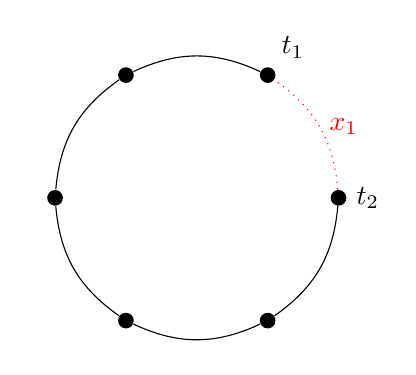
\begin{tikzpicture}[baseline, scale=0.9]
 	 % Set the radius of the imaginary circle
 	 \def\radius{2cm}
 	 % Define the array of labels
 	 \def\labels{{2, 1, 5, 6, 3, 4}}
  
	  % Calculate the position of each point on the circle
 	 \foreach \i in {1,...,6} {
 	   \pgfmathsetmacro\label{\labels[\i - 1]}
 	   \ifthenelse{\label < 3}
 		    {\draw ({360/6 * (\i - 1)}:\radius) node[circle, fill, inner sep=2pt, label={360/6 * (\i - 1):$t_{\label}$}] (t\label) {};}
			{\draw ({360/6 * (\i - 1)}:\radius) node[circle, fill, inner sep=2pt, label={360/6 * (\i - 1)}:] (t\label) {};}
 	 }
 	 
 	 % Draw curved edges between specific points
 	 \draw (t4) to[out=35,in=-95] (t2);
 	 \draw (t1) to[out=155,in=25] (t5);
 	 \draw (t6) to[out=-85,in=145] (t3);
	 \draw (t5) to[out=215,in=85] (t6);
 	 \draw (t3) to[out=-25,in=205] (t4);

  
	 \draw[dotted, red] (t2) to[out=95,in=-35] node[midway, right] {$x_1$} (t1);
	\end{tikzpicture}
	\hspace{25pt}
	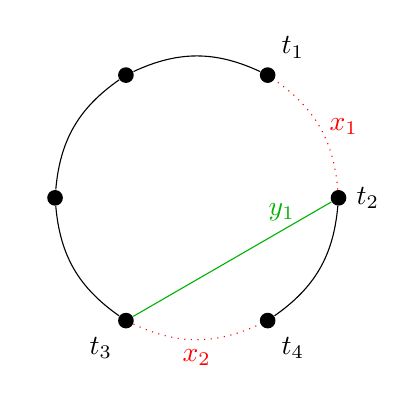
\begin{tikzpicture}[baseline, scale=0.9]
 	 % Set the radius of the imaginary circle
 	 \def\radius{2cm}
 	 % Define the array of labels
 	 \def\labels{{2, 1, 5, 6, 3, 4}}
  
	  % Calculate the position of each point on the circle
 	 \foreach \i in {1,...,6} {
 	   \pgfmathsetmacro\label{\labels[\i - 1]}
 	   \ifthenelse{\label < 5}
 		    {\draw ({360/6 * (\i - 1)}:\radius) node[circle, fill, inner sep=2pt, label={360/6 * (\i - 1):$t_{\label}$}] (t\label) {};}
			{\draw ({360/6 * (\i - 1)}:\radius) node[circle, fill, inner sep=2pt, label={360/6 * (\i - 1)}:] (t\label) {};}
 	 }
 	 
 	 % Draw curved edges between specific points
 	 \draw (t4) to[out=35,in=-95] (t2);
 	 \draw (t1) to[out=155,in=25] (t5);
 	 \draw (t6) to[out=-85,in=145] (t3);
	 \draw (t5) to[out=215,in=85] (t6);

  
	 \draw[dotted, red] (t2) to[out=95,in=-35] node[midway, right] {$x_1$} (t1);
 	 \draw[dotted, red] (t3)to[out=-25,in=205] node[midway, below] {$x_2$} (t4);
  
	 \draw[green!70!black] (t2) to[] node[near start, above] {$y_1$} (t3);
	\end{tikzpicture}
	
	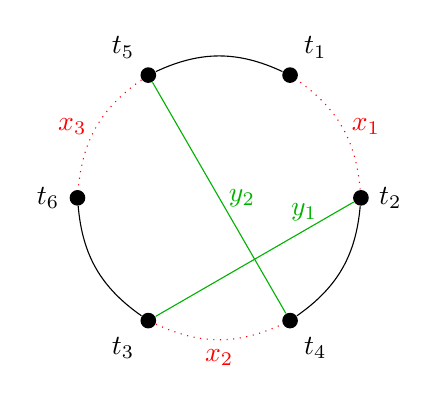
\begin{tikzpicture}[baseline, scale=0.9]
 	 % Set the radius of the imaginary circle
 	 \def\radius{2cm}
 	 % Define the array of labels
 	 \def\labels{{2, 1, 5, 6, 3, 4}}
  
	  % Calculate the position of each point on the circle
 	 \foreach \i in {1,...,6} {
 	   \pgfmathsetmacro\label{\labels[\i - 1]}
 	   {\draw ({360/6 * (\i - 1)}:\radius) node[circle, fill, inner sep=2pt, label={360/6 * (\i - 1):$t_{\label}$}] (t\label) {};}
 	 }
 	 
 	 % Draw curved edges between specific points
 	 \draw (t4) to[out=35,in=-95] (t2);
 	 \draw (t1) to[out=155,in=25] (t5);
 	 \draw (t6) to[out=-85,in=145] (t3);

  
	 \draw[dotted, red] (t2) to[out=95,in=-35] node[midway, right] {$x_1$} (t1);
	 \draw[dotted, red] (t5) to[out=215,in=85] node[midway, left] {$x_3$} (t6);
 	 \draw[dotted, red] (t3)to[out=-25,in=205] node[midway, below] {$x_2$} (t4);
  
	 \draw[green!70!black] (t2) to[] node[near start, above] {$y_1$} (t3);
 	 \draw[green!70!black] (t4) to[] node[midway, right] {$y_2$} (t5);
	\end{tikzpicture}
	\hspace{25pt}
	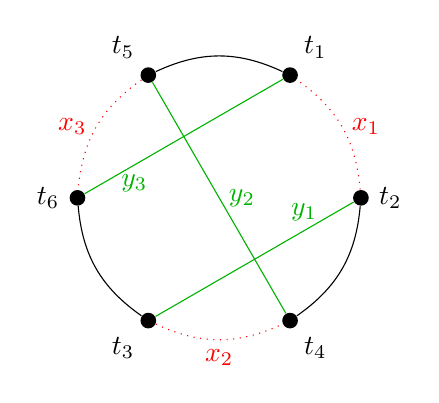
\begin{tikzpicture}[baseline, scale=0.9]
 	 % Set the radius of the imaginary circle
 	 \def\radius{2cm}
 	 % Define the array of labels
 	 \def\labels{{2, 1, 5, 6, 3, 4}}
  
	  % Calculate the position of each point on the circle
 	 \foreach \i in {1,...,6} {
 	   \pgfmathsetmacro\label{\labels[\i - 1]}
 	   \draw ({360/6 * (\i - 1)}:\radius) node[circle, fill, inner sep=2pt, label={360/6 * (\i - 1):$t_{\label}$}] (t\label) {};
 	 }
  
 	 % Draw curved edges between specific points
 	 \draw (t4) to[out=35,in=-95] (t2);
 	 \draw (t1) to[out=155,in=25] (t5);
 	 \draw (t6) to[out=-85,in=145] (t3);

  
	 \draw[dotted, red] (t2) to[out=95,in=-35] node[midway, right] {$x_1$} (t1);
	 \draw[dotted, red] (t5) to[out=215,in=85] node[midway, left] {$x_3$} (t6);
 	 \draw[dotted, red] (t3)to[out=-25,in=205] node[midway, below] {$x_2$} (t4);
  
 	 \draw[green!70!black] (t1) to[] node[near end, below] {$y_3$} (t6);
	 \draw[green!70!black] (t2) to[] node[near start, above] {$y_1$} (t3);
 	 \draw[green!70!black] (t4) to[] node[midway, right] {$y_2$} (t5);
	\end{tikzpicture}
\end{center}
\captionof{figure}{Sekvenční hledání hran}\leavevmode\newline

Sekvenčnost tedy znamená, že zrušíme-li hranu $x_i = (t_i, t_{i+1})$, pak přidaná hrana s ní bude druhý bod sdílet, tedy $y_i = (t_{i+1}, t_{i+2})$, a následně zrušená hrana bude mít zase tvar $x_{i+1} = (t_{i+2}, t_{i+3})$. Poslední přidaná hrana potom bude $y_k = (t_{2i}, t_1)$.

\hspace{6.5mm}Další podmínky kladené na vybírané hrany jsou již zmíněné \textit{pravidlo disjunkce}, kde $\{x_1, x_2, ... x_k\} \cap \{y_1, y_2, ... y_k\} = \emptyset$, \textit{podmínka proveditelnosti} a námi určené \textit{pravidlo výběru}.

\hspace{6.5mm}Abychom mohli kdykoli s hledáním skončit, musíme pro každý pár ověřit, že po přidání hrany $y_k = (t_{2i}, t_1)$ nám vznikne znovu cesta. V implementaci knihovny je toto řešeno následovně.

\hspace{6.5mm}Při každé iteraci je k dispozici cesta, která vznikla záměnou $\{x_1, x_2, ... x_{i-1}\}$ za $\{y_1, y_2, ... y_{enc}\}$. Navíc se ještě udržuje hodnota $t_1$ (ta se v průběhu nemění) a~$t_{2(i-1)}$.

\hspace{6.5mm}Odstraněním $y_{enc} = (t_1, t_{2(i-1)})$ kružnici otevřeme. Nyní další rušená hrana $x_i = (t_{2i-1}, t_{2i})$ musí mít stejný směr jako hrana $(t_{2(i-1)}, t_1)$. Při obrácené orientaci by došlo k rozdělení grafu na dvě komponenty.

\hspace{6.5mm}Jelikož klademe podmínku, že hrany jsou hledané sekvenčně, tak přidaná hrana, pak bude mít tvar $y_{i-1} = (t_{2(i-1)}, t_{2i-1})$. Nakonec cestu opět uzavřeme přidáním hrany $y_{enc} = (t_1, t_{2i})$.


\begin{center}
	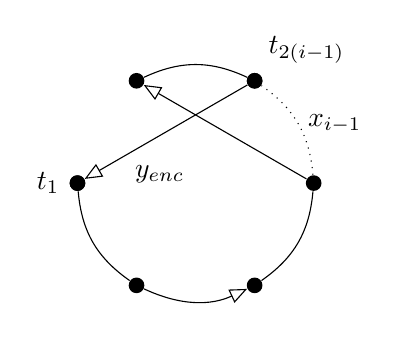
\begin{tikzpicture}[baseline]
 	 % Set the radius of the imaginary circle
 	 \def\radius{1.5cm}
  
	  % Calculate the position of each point on the circle
 	 \foreach \i in {1,...,6} {
 	 	\draw ({360/6 * (\i - 1)}:\radius) node[circle, fill, inner sep=2pt, label={360/6 * (\i - 1)}:] (t\i) {};
 	 }
 	 
 	 \draw ({360/6 * (2 - 1)}:\radius) node[circle, fill, inner sep=2pt, label={360/6 * (2 - 1)}:$t_{2(i-1)}$] (label) {};
 	 \draw ({360/6 * (4 - 1)}:\radius) node[circle, fill, inner sep=2pt, label={360/6 * (4 - 1)}:$t_{1}$] (label) {};
  
 	 % Draw curved edges between specific points
	 \draw[dotted] (t1) to[out=95,in=-35] node[midway, right] {$x_{i-1}$} (t2);
 	 \draw (t2) to[out=155,in=25] (t3);
	 %\draw (t3) to[out=215,in=85] (t4);
 	 \draw (t4) to[out=-85,in=145] (t5);
 	 \draw[->, >=open triangle 45] (t5) to[out=-25,in=205] (t6);
 	 \draw (t6) to[out=35,in=-95] (t1);
 	 
 	 \draw ({360/6 * (1.5 - 1)}:\radius) ;
  
 	 \draw[->, >=open triangle 45] (t2) to[] node[near end, below right] {$y_{enc}$} (t4);
 	 \draw[->, >=open triangle 45] (t1) to[] (t3);
 	 
	\end{tikzpicture}
	%
	%###################################################################################
	%
	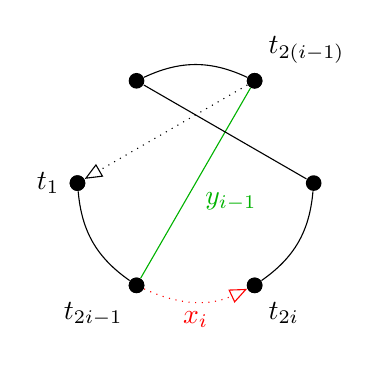
\begin{tikzpicture}[baseline]
 	 % Set the radius of the imaginary circle
 	 \def\radius{1.5cm}
  
	  % Calculate the position of each point on the circle
 	 \foreach \i in {1,...,6} {
 	 	\draw ({360/6 * (\i - 1)}:\radius) node[circle, fill, inner sep=2pt, label={360/6 * (\i - 1)}:] (t\i) {};
 	 }
 	 
 	 \draw ({360/6 * (2 - 1)}:\radius) node[circle, fill, inner sep=2pt, label={360/6 * (2 - 1)}:$t_{2(i-1)}$] (label) {};
 	 \draw ({360/6 * (4 - 1)}:\radius) node[circle, fill, inner sep=2pt, label={360/6 * (4 - 1)}:$t_{1}$] (label) {};
 	 \draw ({360/6 * (5 - 1)}:\radius) node[circle, fill, inner sep=2pt, label={360/6 * (5 - 1)}:$t_{2i-1}$] (label) {};
 	 \draw ({360/6 * (6 - 1)}:\radius) node[circle, fill, inner sep=2pt, label={360/6 * (6 - 1)}:$t_{2i}$] (label) {};
  
 	 % Draw curved edges between specific points
	 %\draw[dotted] (t1) to[out=95,in=-35] (t2);
 	 \draw (t2) to[out=155,in=25] (t3);
	 %\draw (t3) to[out=215,in=85] (t4);
 	 \draw (t4) to[out=-85,in=145] (t5);
 	 \draw[->, >=open triangle 45, dotted, red] (t5) to[out=-25,in=205] node[below] {$x_{i}$}  (t6);
 	 \draw (t6) to[out=35,in=-95] (t1);
 	 
 	 %\draw ({360/6 * (1.5 - 1)}:\radius) node[above, right] {$x_{i-1}$};
  
 	 \draw[->, >=open triangle 45, dotted] (t2) to[] (t4);
 	 \draw[green!70!black] (t2) to[] node[midway, below right] {$y_{i-1}$} (t5);
 	 \draw (t3) to[] (t1);
 	 
	\end{tikzpicture}
	%
	%###################################################################################
	%
	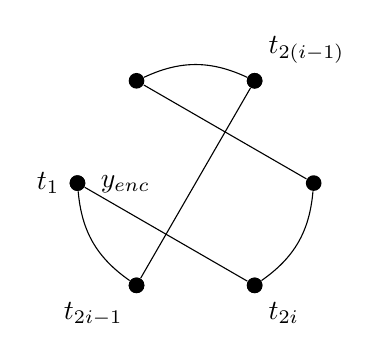
\begin{tikzpicture}[baseline]
 	 % Set the radius of the imaginary circle
 	 \def\radius{1.5cm}
  
	  % Calculate the position of each point on the circle
 	 \foreach \i in {1,...,6} {
 	 	\draw ({360/6 * (\i - 1)}:\radius) node[circle, fill, inner sep=2pt, label={360/6 * (\i - 1)}:] (t\i) {};
 	 }
 	 
 	 \draw ({360/6 * (2 - 1)}:\radius) node[circle, fill, inner sep=2pt, label={360/6 * (2 - 1)}:$t_{2(i-1)}$] (label) {};
 	 \draw ({360/6 * (4 - 1)}:\radius) node[circle, fill, inner sep=2pt, label={360/6 * (4 - 1)}:$t_{1}$] (label) {};
 	 \draw ({360/6 * (5 - 1)}:\radius) node[circle, fill, inner sep=2pt, label={360/6 * (5 - 1)}:$t_{2i-1}$] (label) {};
 	 \draw ({360/6 * (6 - 1)}:\radius) node[circle, fill, inner sep=2pt, label={360/6 * (6 - 1)}:$t_{2i}$] (label) {};
  
 	 % Draw curved edges between specific points
	 %\draw (t1) to[out=95,in=-35] (t2); 	 
 	 %\draw[dotted] (t1) to[out=95,in=-35] (t2);
 	 \draw (t2) to[out=155,in=25] (t3);
	 %\draw (t3) to[out=215,in=85] (t4);
 	 \draw (t4) to[out=-85,in=145] (t5);
 	 %\draw[dotted, red] (t5) to[out=-25,in=205] node[below] {$x_{i}$}  (t6);
 	 \draw (t6) to[out=35,in=-95] (t1);
 	 
 	 %\draw ({360/6 * (1.5 - 1)}:\radius) node[above, right] {$x_{i-1}$};
  
 	 \draw (t2) to[] (t5);
 	 \draw (t4) to[] node[near start, above=3pt] {$y_{enc}$} (t6);
 	 \draw (t3) to[] (t1);
 	 
	\end{tikzpicture}
\end{center}
\captionof{figure}{Pár vyhovující podmínce proveditelnosti}\leavevmode\newline


\begin{center}
	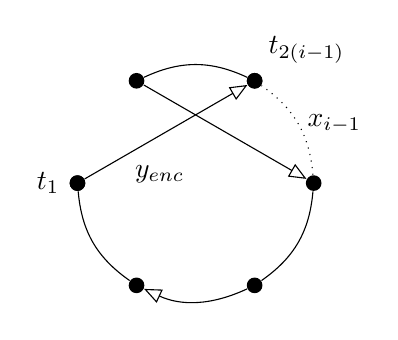
\begin{tikzpicture}[baseline]
 	 % Set the radius of the imaginary circle
 	 \def\radius{1.5cm}
  
	  % Calculate the position of each point on the circle
 	 \foreach \i in {1,...,6} {
 	 	\draw ({360/6 * (\i - 1)}:\radius) node[circle, fill, inner sep=2pt, label={360/6 * (\i - 1)}:] (t\i) {};
 	 }
 	 
 	 \draw ({360/6 * (2 - 1)}:\radius) node[circle, fill, inner sep=2pt, label={360/6 * (2 - 1)}:$t_{2(i-1)}$] (label) {};
 	 \draw ({360/6 * (4 - 1)}:\radius) node[circle, fill, inner sep=2pt, label={360/6 * (4 - 1)}:$t_{1}$] (label) {};
  
 	 % Draw curved edges between specific points
	 \draw[dotted] (t1) to[out=95,in=-35] (t2);
 	 \draw (t2) to[out=155,in=25] (t3);
	 %\draw (t3) to[out=215,in=85] (t4);
 	 \draw (t4) to[out=-85,in=145] (t5);
 	 \draw[->, >=open triangle 45] (t6) to[out=205,in=-25] (t5);
 	 \draw (t6) to[out=35,in=-95] (t1);
 	 
 	 \draw ({360/6 * (1.5 - 1)}:\radius) node[above, right] {$x_{i-1}$};
  
 	 \draw[->, >=open triangle 45] (t4) to[] node[near start, below right] {$y_{enc}$} (t2);
 	 \draw[->, >=open triangle 45] (t3) to[] (t1);
 	 
	\end{tikzpicture}
	%
	%###################################################################################
	%
	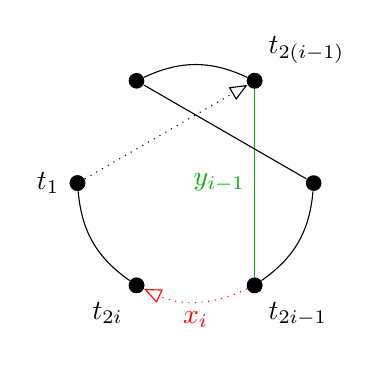
\begin{tikzpicture}[baseline]
 	 % Set the radius of the imaginary circle
 	 \def\radius{1.5cm}
  
	  % Calculate the position of each point on the circle
 	 \foreach \i in {1,...,6} {
 	 	\draw ({360/6 * (\i - 1)}:\radius) node[circle, fill, inner sep=2pt, label={360/6 * (\i - 1)}:] (t\i) {};
 	 }
 	 
 	 \draw ({360/6 * (2 - 1)}:\radius) node[circle, fill, inner sep=2pt, label={360/6 * (2 - 1)}:$t_{2(i-1)}$] (label) {};
 	 \draw ({360/6 * (4 - 1)}:\radius) node[circle, fill, inner sep=2pt, label={360/6 * (4 - 1)}:$t_{1}$] (label) {};
 	 \draw ({360/6 * (5 - 1)}:\radius) node[circle, fill, inner sep=2pt, label={360/6 * (5 - 1)}:$t_{2i}$] (label) {};
 	 \draw ({360/6 * (6 - 1)}:\radius) node[circle, fill, inner sep=2pt, label={360/6 * (6 - 1)}:$t_{2i-1}$] (label) {};
  
 	 % Draw curved edges between specific points
	 %\draw[dotted] (t1) to[out=95,in=-35] (t2);
 	 \draw (t2) to[out=155,in=25] (t3);
	 %\draw (t3) to[out=215,in=85] (t4);
 	 \draw (t4) to[out=-85,in=145] (t5);
 	 \draw[->, >=open triangle 45, dotted, red] (t6) to[out=205,in=-25] node[below] {$x_{i}$}  (t5);
 	 \draw (t6) to[out=35,in=-95] (t1);
 	 
 	 %\draw ({360/6 * (1.5 - 1)}:\radius) node[above, right] {$x_{i-1}$};
  
 	 \draw[->, >=open triangle 45, dotted] (t4) to[] (t2);
 	 \draw[green!70!black] (t2) to[] node[midway, left] {$y_{i-1}$} (t6);
 	 \draw (t3) to[] (t1);
 	 
	\end{tikzpicture}
	%
	%###################################################################################
	%
	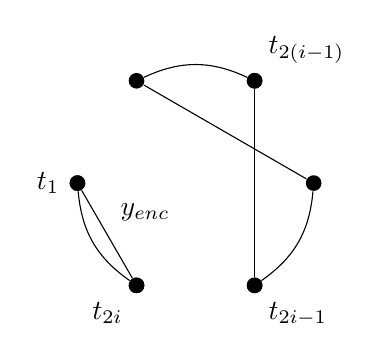
\begin{tikzpicture}[baseline]
 	 % Set the radius of the imaginary circle
 	 \def\radius{1.5cm}
  
	  % Calculate the position of each point on the circle
 	 \foreach \i in {1,...,6} {
 	 	\draw ({360/6 * (\i - 1)}:\radius) node[circle, fill, inner sep=2pt, label={360/6 * (\i - 1)}:] (t\i) {};
 	 }
 	 
 	 \draw ({360/6 * (2 - 1)}:\radius) node[circle, fill, inner sep=2pt, label={360/6 * (2 - 1)}:$t_{2(i-1)}$] (label) {};
 	 \draw ({360/6 * (4 - 1)}:\radius) node[circle, fill, inner sep=2pt, label={360/6 * (4 - 1)}:$t_{1}$] (label) {};
 	 \draw ({360/6 * (5 - 1)}:\radius) node[circle, fill, inner sep=2pt, label={360/6 * (5 - 1)}:$t_{2i}$] (label) {};
 	 \draw ({360/6 * (6 - 1)}:\radius) node[circle, fill, inner sep=2pt, label={360/6 * (6 - 1)}:$t_{2i-1}$] (label) {};
  
 	 % Draw curved edges between specific points
	 %\draw (t1) to[out=95,in=-35] (t2); 	 
 	 %\draw[dotted] (t1) to[out=95,in=-35] (t2);
 	 \draw (t2) to[out=155,in=25] (t3);
	 %\draw (t3) to[out=215,in=85] (t4);
 	 \draw (t4) to[out=-85,in=145] (t5);
 	 %\draw[dotted, red] (t5) to[out=-25,in=205] node[below] {$x_{i}$}  (t6);
 	 \draw (t6) to[out=35,in=-95] (t1);
 	 
 	 %\draw ({360/6 * (1.5 - 1)}:\radius) node[above, right] {$x_{i-1}$};
  
 	 \draw (t2) to[] (t6);
 	 \draw (t4) to[] node[midway, above right=2pt] {$y_{enc}$} (t5);
 	 \draw (t3) to[] (t1);
 	 
	\end{tikzpicture}
\end{center}
\captionof{figure}{Pár nevyhovující podmínce proveditelnosti}\leavevmode\newline

Nyní se podíváme na to, jak identifikovat aktuálně nejvýhodnější pár k výměně. Přirozeně se naskýtá možnost vybrat takové hrany  $x_{i}$, $y_i$, pro které je $|x_i| - |y_{i}|$ mezi ostatními páry maximální. Právě tohoto \textit{pravidla výběru} se využívá.

\hspace{6.5mm}Problémem ale může být to, že v momentě, kdy vybereme takový pár, tak nebere v úvahu délku $x_{i+1}$. Tohle není ideální, protože $x_{i+1}$ může být výhodná hrana. Navíc se začneme omezovat na lokání informaci o nejbližším vrcholu k $t_{2i}$. Dobrou vylepšením algoritmu je tedy neposuzovat páry jen na základě rozdílu jejich délek, ale i délky $x_{i+1}$.

\hspace{6.5mm}Zbývá nám ještě definovat ziskovou funkci $G_i$. Snadno se nabízí následná definice
$$G_i = \sum_{j=1}^{i}g_j = \sum_{j=1}^{i}{(|x_j| - |y_j|)}$$

\hspace{6.5mm}Nakonec nám ještě musíme určit, za jakých podmínek již se zkracováním cesty přestaneme. Hledání přirozeně přestane, dojdou-li páry, které by vyhovovaly předešle definovaným podmínkám a pravidlům. Pro naši \textit{ukončovací podmínku} si zavedeme proměnnou $G^*$, která bude vyjadřovat největší nalezené zlepšení cesty. Uvědomme si, že $G^* \ne G_k$. Nejedná se totiž o zisk z vyměněných párů, ale o skutečné zkrácení cesty. Tuto hodnotu zjistíme pro $i$-tou iteraci následovně $G_{i-1} + |y_{enc}|$, kde $y_{enc}= (t_{2i}, t_1)$. Čili-že hrana $y_{enc}$ uzavírá cestu, kde je poslední odstraněnou hranou $x_i$. Samotná ukončovací podmínka pak bude $G_i \le G^*$.

\hspace{6.5mm}Nyní už si můžeme ukázat upravenou verzi Keringhan - Lin pro TSP.
\newline

{\LinesNumbered\SetAlgoNoLine\
\begin{algorithm}[H]
\SetKwRepeat{Do}{do}{while}%
$T \leftarrow$ pseudorandom solution\;
$T' \leftarrow T$\;
$k = 0$\;
$i = 0$\;
$G^* = 0$ \tcp*[h]{best improvement}\;
\Do {$G^* > 0$}
{
$i \leftarrow i + 1$\;
find pair $x_{i} = (t_{2i-1}, t_{2i}), y_i = (t_{2i}, t_{2i+1})$ for which:
{\begin{itemize}
\item[a)] $x_{i} \notin \{y_1, y_2,... y_i\}$ and  $y_i \notin \{x_1, x_2,... x_i\}$ 
\item[b)] $T - \{x_1, x_2,... x_i\} \cup \{y_1, y_2,... y_i\}$ is a tour
\item[c)] $|x_{i}| - |y_i|$ is maximal between such pairs
\end{itemize}}
\If {no $x_{i}, y_i$ were found}
	{\textbf{break}\;}
\If {$G_{i-1} + c_{t_{2i},t_1} > G^*$}
	{$k \leftarrow i$\;
	 $G^* = G_{i-1} + c_{t_{2i},t_1}$\;}
\If {$G_i \le G^*$}
	{\textbf{break}\;}
}
$T' \leftarrow (T - \{x_1, x_2, ..., x_k\}) \cup \{y_1, y_2, ..., y_k\}$\;
\Return $T'$\;
\caption{Keringhan - Lin algoritmus pro TSP}
\end{algorithm}}\leavevmode\newline

Co pseudokód neukazuje je omezený backtracking, který se provádí v případě, že $G^* = 0$. V takovém případě se na první a druhé úrovni zkoušejí ostatní možnosti za jednotlivé hrany. Tedy nejdříve budeme zkoušet alternativní $y_2$ (postupně podle sestupné hodnoty $|x_2| - |y_2|$), ve chvíli, kdy jsou všechny možnosti vyčerpány, se zkusí použít alternativní $x_2$ (tento případ je složitější). Takto se pokračuje i se všemi $y_1$, $x_1$ a $t_1$. V momentě, kdy nám žádná ze záměn nepřinese zlepšení, algoritmus končí a vrátí upravenou cestu.

\hspace{6.5mm}Zřejmě kdybychom prováděli takovýto backtracking na každé úrovni, tak bychom byli schopni nalézt optimální řešení. To by ale trvalo nesmírně dlouho. Najít zlatou střední cestu mezi optimalitou a rychlostí je klíčové. Experimenty ukazují, že nezkoušíme-li všechna $y_1$, $y_2$ tak za mírné zhoršení efektivity dostaneme o kratší výpočetní čas.

\hspace{6.5mm}Vraťme se nyní ještě k problému s alternativní volbou $x_2$. Pro tuto hranu máme jistě dvě volby. Abychom mohli cestu uzavřít musí se $t_4$ nacházet mezi $t_2$ a $t_3$. V případě, že to tak není bychom cestu přidáním $y_{enc}$ místo uzavření rozdělili na dvě komponenty.

\begin{center}
	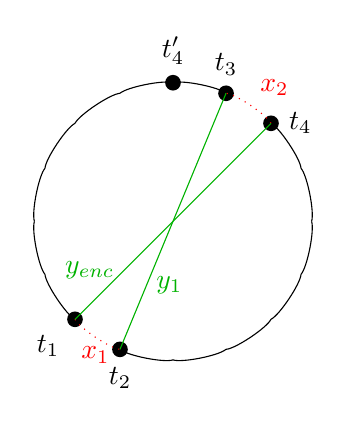
\begin{tikzpicture}[scale=0.88]
 	 % Set the radius of the imaginary circle
 	 \def\radius{2cm}
  
	  % Calculate the position of each point on the circle
 	 \foreach \i in {1,...,16} {
 	 	\coordinate (t\i) at ({360/16 * (\i - 1)}:\radius);
 	 }
 	 
 	 \draw ({360/16 * 2}:\radius) node[circle, fill, inner sep=2pt, label={right:$t_4$}] {};
 	 \draw ({360/16 * 3}:\radius) node[circle, fill, inner sep=2pt, label={above:$t_3$}] {};
 	 \draw ({360/16 * 4}:\radius) node[circle, fill, inner sep=2pt, label={above:$t_4'$}] {};
 	 \draw ({360/16 * 10}:\radius) node[circle, fill, inner sep=2pt, label={below left:$t_1$}] {};
 	 \draw ({360/16 * 11}:\radius) node[circle, fill, inner sep=2pt, label={below:$t_2$}] {};
  
 	 % Draw curved edges between specific points
	 \draw[bend right=30, looseness=0.45] (t1) to[] (t2);
 	 \draw[bend right=30, looseness=0.45] (t2) to[] (t3);
	 \draw[dotted, red, bend right=30, looseness=0.45] (t3) to[] node[above right] {$x_2$} (t4);
 	 \draw[bend right=30, looseness=0.45] (t4) to[] (t5);
 	 \draw[bend right=30, looseness=0.45] (t5) to[] (t6);
 	 \draw[bend right=30, looseness=0.45] (t6) to[] (t7);
 	 \draw[bend right=30, looseness=0.45] (t7) to[] (t8);
	 \draw[bend right=30, looseness=0.45] (t8) to[] (t9);
 	 \draw[bend right=30, looseness=0.45] (t9) to[] (t10);
 	 \draw[bend right=30, looseness=0.45] (t10) to[] (t11);
 	 \draw[dotted, red, bend right=30, looseness=0.45] (t11) to[] node[below, midway] {$x_1$}  (t12);
 	 \draw[bend right=30, looseness=0.45] (t12) to[] (t13);
 	 \draw[bend right=30, looseness=0.45] (t13) to[] (t14);
 	 \draw[bend right=30, looseness=0.45] (t14) to[] (t15);
 	 \draw[bend right=30, looseness=0.45] (t15) to[] (t16);
 	 \draw[bend right=30, looseness=0.45] (t16) to[] (t1);

 	 \draw[green!70!black] (t12) to[] node[near start, right] {$y_1$} (t4);
 	 \draw[green!70!black] (t11) to[] node[near start , left] {$y_{enc}$} (t3);
	\end{tikzpicture}
	\hspace{50pt}
	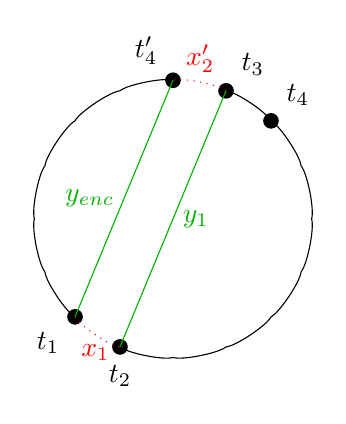
\begin{tikzpicture}[scale=0.88]
 	 % Set the radius of the imaginary circle
 	 \def\radius{2cm}
  
	  % Calculate the position of each point on the circle
 	 \foreach \i in {1,...,16} {
 	 	\coordinate (t\i) at ({360/16 * (\i - 1)}:\radius);
 	 }
 	 
 	 \draw ({360/16 * 2}:\radius) node[circle, fill, inner sep=2pt, label={above right:$t_4$}] {};
 	 \draw ({360/16 * 3}:\radius) node[circle, fill, inner sep=2pt, label={above right :$t_3$}] {};
 	 \draw ({360/16 * 4}:\radius) node[circle, fill, inner sep=2pt, label={above left:$t_4'$}] {};
 	 
 	 \draw ({360/16 * 10}:\radius) node[circle, fill, inner sep=2pt, label={below left:$t_1$}] {};
 	 \draw ({360/16 * 11}:\radius) node[circle, fill, inner sep=2pt, label={below:$t_2$}] {};
  
 	 % Draw curved edges between specific points
	 \draw[bend right=30, looseness=0.45] (t1) to[] (t2);
 	 \draw[bend right=30, looseness=0.45] (t2) to[] (t3);
	 \draw[bend right=30, looseness=0.45] (t3) to[] (t4);
 	 \draw[dotted, red, bend right=30, looseness=0.45] (t4) to[] node[above] {$x_2'$} (t5);
 	 \draw[bend right=30, looseness=0.45] (t5) to[] (t6);
 	 \draw[bend right=30, looseness=0.45] (t6) to[] (t7);
 	 \draw[bend right=30, looseness=0.45] (t7) to[] (t8);
	 \draw[bend right=30, looseness=0.45] (t8) to[] (t9);
 	 \draw[bend right=30, looseness=0.45] (t9) to[] (t10);
 	 \draw[bend right=30, looseness=0.45] (t10) to[] (t11);
 	 \draw[dotted, red, bend right=30, looseness=0.45] (t11) to[] node[midway, below] {$x_1$}  (t12);
 	 \draw[bend right=30, looseness=0.45] (t12) to[] (t13);
 	 \draw[bend right=30, looseness=0.45] (t13) to[] (t14);
 	 \draw[bend right=30, looseness=0.45] (t14) to[] (t15);
 	 \draw[bend right=30, looseness=0.45] (t15) to[] (t16);
 	 \draw[bend right=30, looseness=0.45] (t16) to[] (t1);

 	 \draw[green!70!black] (t12) to[] node[midway , right] {$y_1$} (t4);
 	 \draw[green!70!black] (t11) to[] node[midway , left] {$y_{enc}$} (t5);
	\end{tikzpicture}
\end{center}
\captionof{figure}{Problém alternativního $x_2$}\leavevmode\newline

Abychom i přes to mohli použít druhou volbu $x_2$ svolíme na chvíli z podmínky proveditelnosti a budeme pokračovat v hledání hran následovně. První možností je vybrat $y_2$ tak, že $t_5$ leží mezi $t_3$ a $t_2$. $t_6$ pak může být na libovolné straně od $t_5$. V tuto chvíli je již možné cestu řádně uzavřít.

\begin{center}
	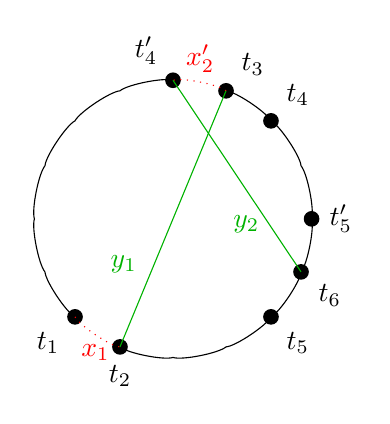
\begin{tikzpicture}[scale=0.88]
 	 % Set the radius of the imaginary circle
 	 \def\radius{2cm}
  
	  % Calculate the position of each point on the circle
 	 \foreach \i in {1,...,16} {
 	 	\coordinate (t\i) at ({360/16 * (\i - 1)}:\radius);
 	 }
 	 
 	 
 	 \draw ({360/16 * 2}:\radius) node[circle, fill, inner sep=2pt, label={above right:$t_4$}] {};
 	 \draw ({360/16 * 3}:\radius) node[circle, fill, inner sep=2pt, label={above right :$t_3$}] {};
 	 \draw ({360/16 * 4}:\radius) node[circle, fill, inner sep=2pt, label={above left:$t_4'$}] {};
 	 
 	 \draw ({360/16 * 10}:\radius) node[circle, fill, inner sep=2pt, label={below left:$t_1$}] {};
 	 \draw ({360/16 * 11}:\radius) node[circle, fill, inner sep=2pt, label={below:$t_2$}] {};
 	 
 	 \draw ({360/16 * 14}:\radius) node[circle, fill, inner sep=2pt, label={360/16 * 14}:{$t_5$}] {};
 	 \draw ({360/16 * 15}:\radius) node[circle, fill, inner sep=2pt, label={360/16 * 15}:{$t_6$}] {};
 	 \draw ({360/16 * 16}:\radius) node[circle, fill, inner sep=2pt, label={360/16 * 16}:{$t_5'$}] {};
  
 	 % Draw curved edges between specific points
	 \draw[bend right=30, looseness=0.45] (t1) to[] (t2);
 	 \draw[bend right=30, looseness=0.45] (t2) to[] (t3);
	 \draw[bend right=30, looseness=0.45] (t3) to[] (t4);
 	 \draw[dotted, red, bend right=30, looseness=0.45] (t4) to[] node[midway, above] {$x_2'$} (t5);
 	 \draw[bend right=30, looseness=0.45] (t5) to[] (t6);
 	 \draw[bend right=30, looseness=0.45] (t6) to[] (t7);
 	 \draw[bend right=30, looseness=0.45] (t7) to[] (t8);
	 \draw[bend right=30, looseness=0.45] (t8) to[] (t9);
 	 \draw[bend right=30, looseness=0.45] (t9) to[] (t10);
 	 \draw[bend right=30, looseness=0.45] (t10) to[] (t11);
 	 \draw[dotted, red, bend right=30, looseness=0.45] (t11) to[] node[below, midway] {$x_1$}  (t12);
 	 \draw[bend right=30, looseness=0.45] (t12) to[] (t13);
 	 \draw[bend right=30, looseness=0.45] (t13) to[] (t14);
 	 \draw[bend right=30, looseness=0.45] (t14) to[] (t15);
 	 \draw[bend right=30, looseness=0.45] (t15) to[] (t16);
 	 \draw[bend right=30, looseness=0.45] (t16) to[] (t1);

 	 \draw[green!70!black] (t12) to[] node[near start, above left] {$y_1$} (t4);
 	 \draw[green!70!black] (t16) to[] node[near start , left] {$y_2$} (t5);
	\end{tikzpicture}
	\hspace{50pt}
	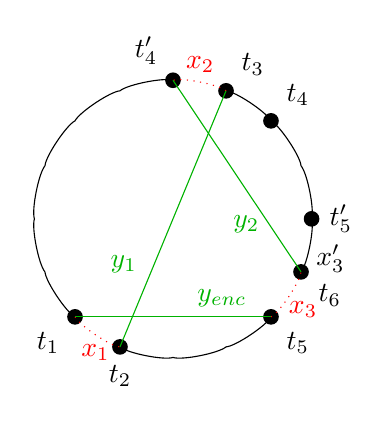
\begin{tikzpicture}[scale=0.88]
 	 % Set the radius of the imaginary circle
 	 \def\radius{2cm}
  
	  % Calculate the position of each point on the circle
 	 \foreach \i in {1,...,16} {
 	 	\coordinate (t\i) at ({360/16 * (\i - 1)}:\radius);
 	 }
 	 
 	 \draw ({360/16 * 2}:\radius) node[circle, fill, inner sep=2pt, label={above right:$t_4$}] {};
 	 \draw ({360/16 * 3}:\radius) node[circle, fill, inner sep=2pt, label={above right :$t_3$}] {};
 	 \draw ({360/16 * 4}:\radius) node[circle, fill, inner sep=2pt, label={above left:$t_4'$}] {};
 	 
 	 \draw ({360/16 * 10}:\radius) node[circle, fill, inner sep=2pt, label={below left:$t_1$}] {};
 	 \draw ({360/16 * 11}:\radius) node[circle, fill, inner sep=2pt, label={below:$t_2$}] {};
 	 
 	 \draw ({360/16 * 14}:\radius) node[circle, fill, inner sep=2pt, label={360/16 * 14}:{$t_5$}] {};
 	 \draw ({360/16 * 15}:\radius) node[circle, fill, inner sep=2pt, label={360/16 * 15}:{$t_6$}] {};
 	 \draw ({360/16 * 16}:\radius) node[circle, fill, inner sep=2pt, label={360/16 * 16}:{$t_5'$}] {};
  
 	 % Draw curved edges between specific points
	 \draw[bend right=30, looseness=0.45] (t1) to[] (t2);
 	 \draw[bend right=30, looseness=0.45] (t2) to[] (t3);
	 \draw[bend right=30, looseness=0.45] (t3) to[] (t4);
 	 \draw[dotted, red, bend right=30, looseness=0.45] (t4) to[] node[midway, above] {$x_2$} (t5);
 	 \draw[bend right=30, looseness=0.45] (t5) to[] (t6);
 	 \draw[bend right=30, looseness=0.45] (t6) to[] (t7);
 	 \draw[bend right=30, looseness=0.45] (t7) to[] (t8);
	 \draw[bend right=30, looseness=0.45] (t8) to[] (t9);
 	 \draw[bend right=30, looseness=0.45] (t9) to[] (t10);
 	 \draw[bend right=30, looseness=0.45] (t10) to[] (t11);
 	 \draw[dotted, red, bend right=30, looseness=0.45] (t11) to[] node[below, midway] {$x_1$} (t12);
 	 \draw[bend right=30, looseness=0.45] (t12) to[] (t13);
 	 \draw[bend right=30, looseness=0.45] (t13) to[] (t14);
 	 \draw[bend right=30, looseness=0.45] (t14) to[] (t15);
 	 \draw[dotted, red, bend right=30, looseness=0.45] (t15) to[] node[right,pos=0.25] {$x_3$} (t16);
 	 \draw[bend right=30, looseness=0.45] (t16) to[] node[right,pos=0.3] {$x_3'$} (t1);

 	 \draw[green!70!black] (t12) to[] node[near start, above left] {$y_1$} (t4);
 	 \draw[green!70!black] (t16) to[] node[near start , left] {$y_2$} (t5);
 	 \draw[green!70!black] (t15) to[] node[near start, above] {$y_{enc}$} (t11);
	\end{tikzpicture}
\end{center}
\captionof{figure}{Alternativní $x_2$ - první možnost cesty}\leavevmode\newline

Druhou možností je zvolit $t_5$ tak, že leží mezi $t_4'$ a $t_1$. $t_6$ se pak musí nacházet mezi $t_6$ a $t_1$. Nakonec $t_7$ musí být mezi $t_3$ a $t_2$ s tím, že volba $t_8$ závisí, zda-li je delší $x_4$ nebo $x_4'$.

\begin{center}
	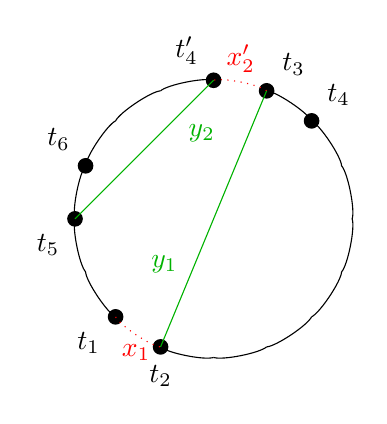
\begin{tikzpicture}[scale=0.88]
 	 % Set the radius of the imaginary circle
 	 \def\radius{2cm}
  
	  % Calculate the position of each point on the circle
 	 \foreach \i in {1,...,16} {
 	 	\coordinate (t\i) at ({360/16 * (\i - 1)}:\radius);
 	 }
 	 
 	 \draw ({360/16 * 2}:\radius) node[circle, fill, inner sep=2pt, label={above right:$t_4$}] {};
 	 \draw ({360/16 * 3}:\radius) node[circle, fill, inner sep=2pt, label={above right :$t_3$}] {};
 	 \draw ({360/16 * 4}:\radius) node[circle, fill, inner sep=2pt, label={above left:$t_4'$}] {};
 	 
 	 \draw ({360/16 * 10}:\radius) node[circle, fill, inner sep=2pt, label={below left:$t_1$}] {};
 	 \draw ({360/16 * 11}:\radius) node[circle, fill, inner sep=2pt, label={below:$t_2$}] {};
 	 
 	 \draw ({360/16 * 7}:\radius) node[circle, fill, inner sep=2pt, label={above left:$t_6$}] {};
 	 \draw ({360/16 * 8}:\radius) node[circle, fill, inner sep=2pt, label={below left:$t_5$}] {};
  
 	 % Draw curved edges between specific points
	 \draw[bend right=30, looseness=0.45] (t1) to[] (t2);
 	 \draw[bend right=30, looseness=0.45] (t2) to[] (t3);
	 \draw[bend right=30, looseness=0.45] (t3) to[] (t4);
 	 \draw[dotted, red, bend right=30, looseness=0.45] (t4) to[] node[midway, above] {$x_2'$} (t5);
 	 \draw[bend right=30, looseness=0.45] (t5) to[] (t6);
 	 \draw[bend right=30, looseness=0.45] (t6) to[] (t7);
 	 \draw[bend right=30, looseness=0.45] (t7) to[] (t8);
	 \draw[bend right=30, looseness=0.45] (t8) to[] (t9);
 	 \draw[bend right=30, looseness=0.45] (t9) to[] (t10);
 	 \draw[bend right=30, looseness=0.45] (t10) to[] (t11);
 	 \draw[dotted, red, bend right=30, looseness=0.45] (t11) to[] node[below, midway] {$x_1$}  (t12);
 	 \draw[bend right=30, looseness=0.45] (t12) to[] (t13);
 	 \draw[bend right=30, looseness=0.45] (t13) to[] (t14);
 	 \draw[bend right=30, looseness=0.45] (t14) to[] (t15);
 	 \draw[bend right=30, looseness=0.45] (t15) to[] (t16);
 	 \draw[bend right=30, looseness=0.45] (t16) to[] (t1);

 	 \draw[green!70!black] (t12) to[] node[near start, above left] {$y_1$} (t4);
 	 \draw[green!70!black] (t9) to[] node[near end, below right] {$y_2$} (t5);
	\end{tikzpicture}
	\hfill
	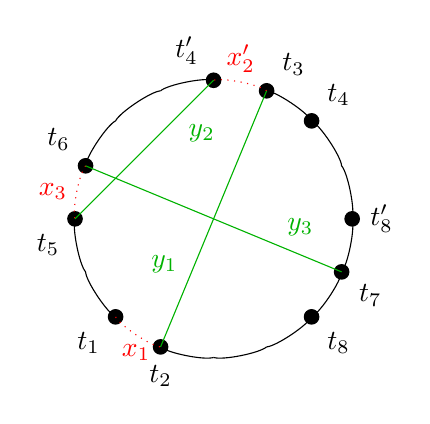
\begin{tikzpicture}[scale=0.88]
 	 % Set the radius of the imaginary circle
 	 \def\radius{2cm}
  
	  % Calculate the position of each point on the circle
 	 \foreach \i in {1,...,16} {
 	 	\coordinate (t\i) at ({360/16 * (\i - 1)}:\radius);
 	 }
 	 
 	 \draw ({360/16 * 2}:\radius) node[circle, fill, inner sep=2pt, label={above right:$t_4$}] {};
 	 \draw ({360/16 * 3}:\radius) node[circle, fill, inner sep=2pt, label={above right :$t_3$}] {};
 	 \draw ({360/16 * 4}:\radius) node[circle, fill, inner sep=2pt, label={above left:$t_4'$}] {};
 	 
 	 \draw ({360/16 * 10}:\radius) node[circle, fill, inner sep=2pt, label={below left:$t_1$}] {};
 	 \draw ({360/16 * 11}:\radius) node[circle, fill, inner sep=2pt, label={below:$t_2$}] {};
 	 
 	 \draw ({360/16 * 7}:\radius) node[circle, fill, inner sep=2pt, label={above left:$t_6$}] {};
 	 \draw ({360/16 * 8}:\radius) node[circle, fill, inner sep=2pt, label={below left:$t_5$}] {};

 	 \draw ({360/16 * 14}:\radius) node[circle, fill, inner sep=2pt, label={360/16 * 14}:{$t_8$}] {};
 	 \draw ({360/16 * 15}:\radius) node[circle, fill, inner sep=2pt, label={360/16 * 15}:{$t_7$}] {};
 	 \draw ({360/16 * 16}:\radius) node[circle, fill, inner sep=2pt, label={360/16 * 16}:{$t_8'$}] {};
  
 	 % Draw curved edges between specific points
	 \draw[bend right=30, looseness=0.45] (t1) to[] (t2);
 	 \draw[bend right=30, looseness=0.45] (t2) to[] (t3);
	 \draw[bend right=30, looseness=0.45] (t3) to[] (t4);
 	 \draw[dotted, red, bend right=30, looseness=0.45] (t4) to[] node[midway, above] {$x_2'$} (t5);
 	 \draw[bend right=30, looseness=0.45] (t5) to[] (t6);
 	 \draw[bend right=30, looseness=0.45] (t6) to[] (t7);
 	 \draw[bend right=30, looseness=0.45] (t7) to[] (t8);
	 \draw[dotted, red, bend right=30, looseness=0.45] (t8) to[] node[left] {$x_3$}  (t9);
 	 \draw[bend right=30, looseness=0.45] (t9) to[] (t10);
 	 \draw[bend right=30, looseness=0.45] (t10) to[] (t11);
 	 \draw[dotted, red, bend right=30, looseness=0.45] (t11) to[] node[below, midway] {$x_1$}  (t12);
 	 \draw[bend right=30, looseness=0.45] (t12) to[] (t13);
 	 \draw[bend right=30, looseness=0.45] (t13) to[] (t14);
 	 \draw[bend right=30, looseness=0.45] (t14) to[] (t15);
 	 \draw[bend right=30, looseness=0.45] (t15) to[] (t16);
 	 \draw[bend right=30, looseness=0.45] (t16) to[] (t1);

 	 \draw[green!70!black] (t12) to[] node[near start, above left] {$y_1$} (t4);
 	 \draw[green!70!black] (t9) to[] node[near end, below right] {$y_2$} (t5);
 	 \draw[green!70!black] (t8) to[] node[near end, above right] {$y_3$} (t16);
	\end{tikzpicture}
	\hfill
	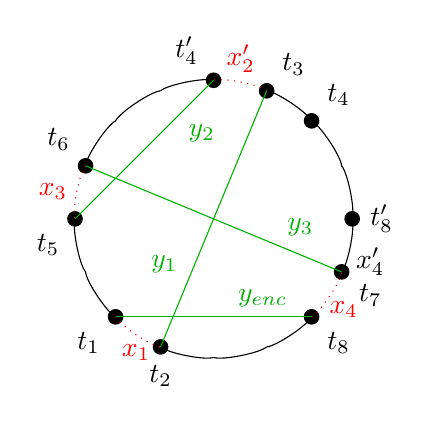
\begin{tikzpicture}[scale=0.88]
 	 % Set the radius of the imaginary circle
 	 \def\radius{2cm}
  
	  % Calculate the position of each point on the circle
 	 \foreach \i in {1,...,16} {
 	 	\coordinate (t\i) at ({360/16 * (\i - 1)}:\radius);
 	 }
 	 
 	 \draw ({360/16 * 2}:\radius) node[circle, fill, inner sep=2pt, label={above right:$t_4$}] {};
 	 \draw ({360/16 * 3}:\radius) node[circle, fill, inner sep=2pt, label={above right :$t_3$}] {};
 	 \draw ({360/16 * 4}:\radius) node[circle, fill, inner sep=2pt, label={above left:$t_4'$}] {};
 	 
 	 \draw ({360/16 * 10}:\radius) node[circle, fill, inner sep=2pt, label={below left:$t_1$}] {};
 	 \draw ({360/16 * 11}:\radius) node[circle, fill, inner sep=2pt, label={below:$t_2$}] {};
 	 
 	 \draw ({360/16 * 7}:\radius) node[circle, fill, inner sep=2pt, label={above left:$t_6$}] {};
 	 \draw ({360/16 * 8}:\radius) node[circle, fill, inner sep=2pt, label={below left:$t_5$}] {};

 	 \draw ({360/16 * 14}:\radius) node[circle, fill, inner sep=2pt, label={360/16 * 14}:{$t_8$}] {};
 	 \draw ({360/16 * 15}:\radius) node[circle, fill, inner sep=2pt, label={360/16 * 15}:{$t_7$}] {};
 	 \draw ({360/16 * 16}:\radius) node[circle, fill, inner sep=2pt, label={360/16 * 16}:{$t_8'$}] {};
 	 % Draw curved edges between specific points
	 \draw[bend right=30, looseness=0.45] (t1) to[] (t2);
 	 \draw[bend right=30, looseness=0.45] (t2) to[] (t3);
	 \draw[bend right=30, looseness=0.45] (t3) to[] (t4);
 	 \draw[dotted, red, bend right=30, looseness=0.45] (t4) to[] node[midway, above] {$x_2'$} (t5);
 	 \draw[bend right=30, looseness=0.45] (t5) to[] (t6);
 	 \draw[bend right=30, looseness=0.45] (t6) to[] (t7);
 	 \draw[bend right=30, looseness=0.45] (t7) to[] (t8);
	 \draw[dotted, red, bend right=30, looseness=0.45] (t8) to[] node[left] {$x_3$}  (t9);
 	 \draw[bend right=30, looseness=0.45] (t9) to[] (t10);
 	 \draw[bend right=30, looseness=0.45] (t10) to[] (t11);
 	 \draw[dotted, red, bend right=30, looseness=0.45] (t11) to[] node[below, midway] {$x_1$} (t12);
 	 \draw[bend right=30, looseness=0.45] (t12) to[] (t13);
 	 \draw[bend right=30, looseness=0.45] (t13) to[] (t14);
 	 \draw[bend right=30, looseness=0.45] (t14) to[] (t15);
 	 \draw[dotted, red, bend right=30, looseness=0.45] (t15) to[] node[near start, right] {$x_4$} (t16);
 	 \draw[bend right=30, looseness=0.45] (t16) to[] node[near start, right] {$x_4'$} (t1);

 	 \draw[green!70!black] (t12) to[] node[near start, above left] {$y_1$} (t4);
 	 \draw[green!70!black] (t9) to[] node[near end, below right] {$y_2$} (t5);
 	 \draw[green!70!black] (t8) to[] node[near end, above right] {$y_3$} (t16);
 	 \draw[green!70!black] (t11) to[] node[near end, above] {$y_{enc}$} (t15);
	\end{tikzpicture}
\end{center}
\captionof{figure}{Alternativní $x_2$ - druhá možnost cesty} \leavevmode\newline

\begin{kiconclusions}
Závěr práce v \uv{českém} jazyce.
\end{kiconclusions}

\begin{kiconclusions}[english]
Thesis conclusions in \uv{English}.
\end{kiconclusions}


%% -------------------------------------------------------------------

%% Sazba volitelného seznamu zkratek, za přílohami.
\printglossary

%% Sazba povinné bibliografie, za přílohami (případně i za seznamem
%% zkratek). Při použití BibLaTeXu použijte makro
%% \printbibliography. jinak prostředí thebibliography. Ne obojí!

%% Sazba i v textu necitovaných zdrojů, při použití
%% BibLaTeXu. Volitelné.
\nocite{*}
%% Vlastní sazba bibliografie při použití BibLaTeXu.
\printbibliography

%% Bibliografie, včetně sazby, při nepoužití BibLaTeXu.
% \begin{thebibliography}{9}
%\bibitem{kniha2} \uppercase{Hawke}, Paul. NanoHttpd: Light-weight HTTP server designed for embedding in other applications. GitHub [online]. 2014-05-12. [cit. 2014-12-06]. Dostupné z: \url{https://github.com/NanoHttpd/nanohttpd}
%
%\bibitem{jeske13} \uppercase{ Jeske}, David; \uppercase{Novák}, Josef. Simple HTTP Server in \csharp: Threaded synchronous HTTP Server abstract class, to respond to HTTP requests. CodeProject: For those who code [online]. 2014-05-24. [cit. 2014-12-06]. Dostupné z: \url{http://www.codeproject.com/Articles/137979/Simple-HTTP-Server-in-C}
%
%\bibitem{uzis2012} \uppercase{ÚSTAV ZDRAVOTNICKÝCH INFORMACÍ A STATISTIKY ČR}. Lékaři, zubní lékaři a farmaceuti 2012 [online]. Praha 2, Palackého náměstí 4: Ústav zdravotnických informací a statistiky ČR, 2012 [cit. 2014-12-06]. ISBN 978-80-7472-089-5. Dostupné z: \url{http://www.uzis.cz/publikace/lekari-zubni-lekari-farmaceuti-2012}
% \end{thebibliography}

%% Sazba volitelného rejstříku, za bibliografií.
\printindex

\listoffigures

\listoftables

\end{document}

%%% Local Variables:
%%% mode: latex
%%% TeX-master: t
%%% End:
